\chapter{Simulation Results}

% TODO: create github repo and put URL in this paragraph
% TODO: if you're not writing the appendix, do not cite it here
In this Chapter, we simulate the CVSM discussed in Chapter
\ref{chap:vsm-modeling} comparing its transient response when different SG
models are used for generating the reference signals. The simulations are
performed in MATLAB using the library GUILDA (Grid and Utility Infrastructure
Linkage Dynamics Analyzer) developed by Ishizaki Lab. Details about the theory
and algorithms for simulation of power systems can be found in
\cite{sauer2017power,ishizaki2020} and are briefly discussed in the Appendix. A simplified
version of GUILDA, with all the codes for generating the results discussed in
this Chapter can be found in a Github repository. 

\section{System under study}

The system under study is the WECC-9 bus system, consisting of three machines,
three loads and three non-unit buses, as illustrated in Figure \ref{fig:WSCC9}.

\begin{figure}[ht!]
    \centering
    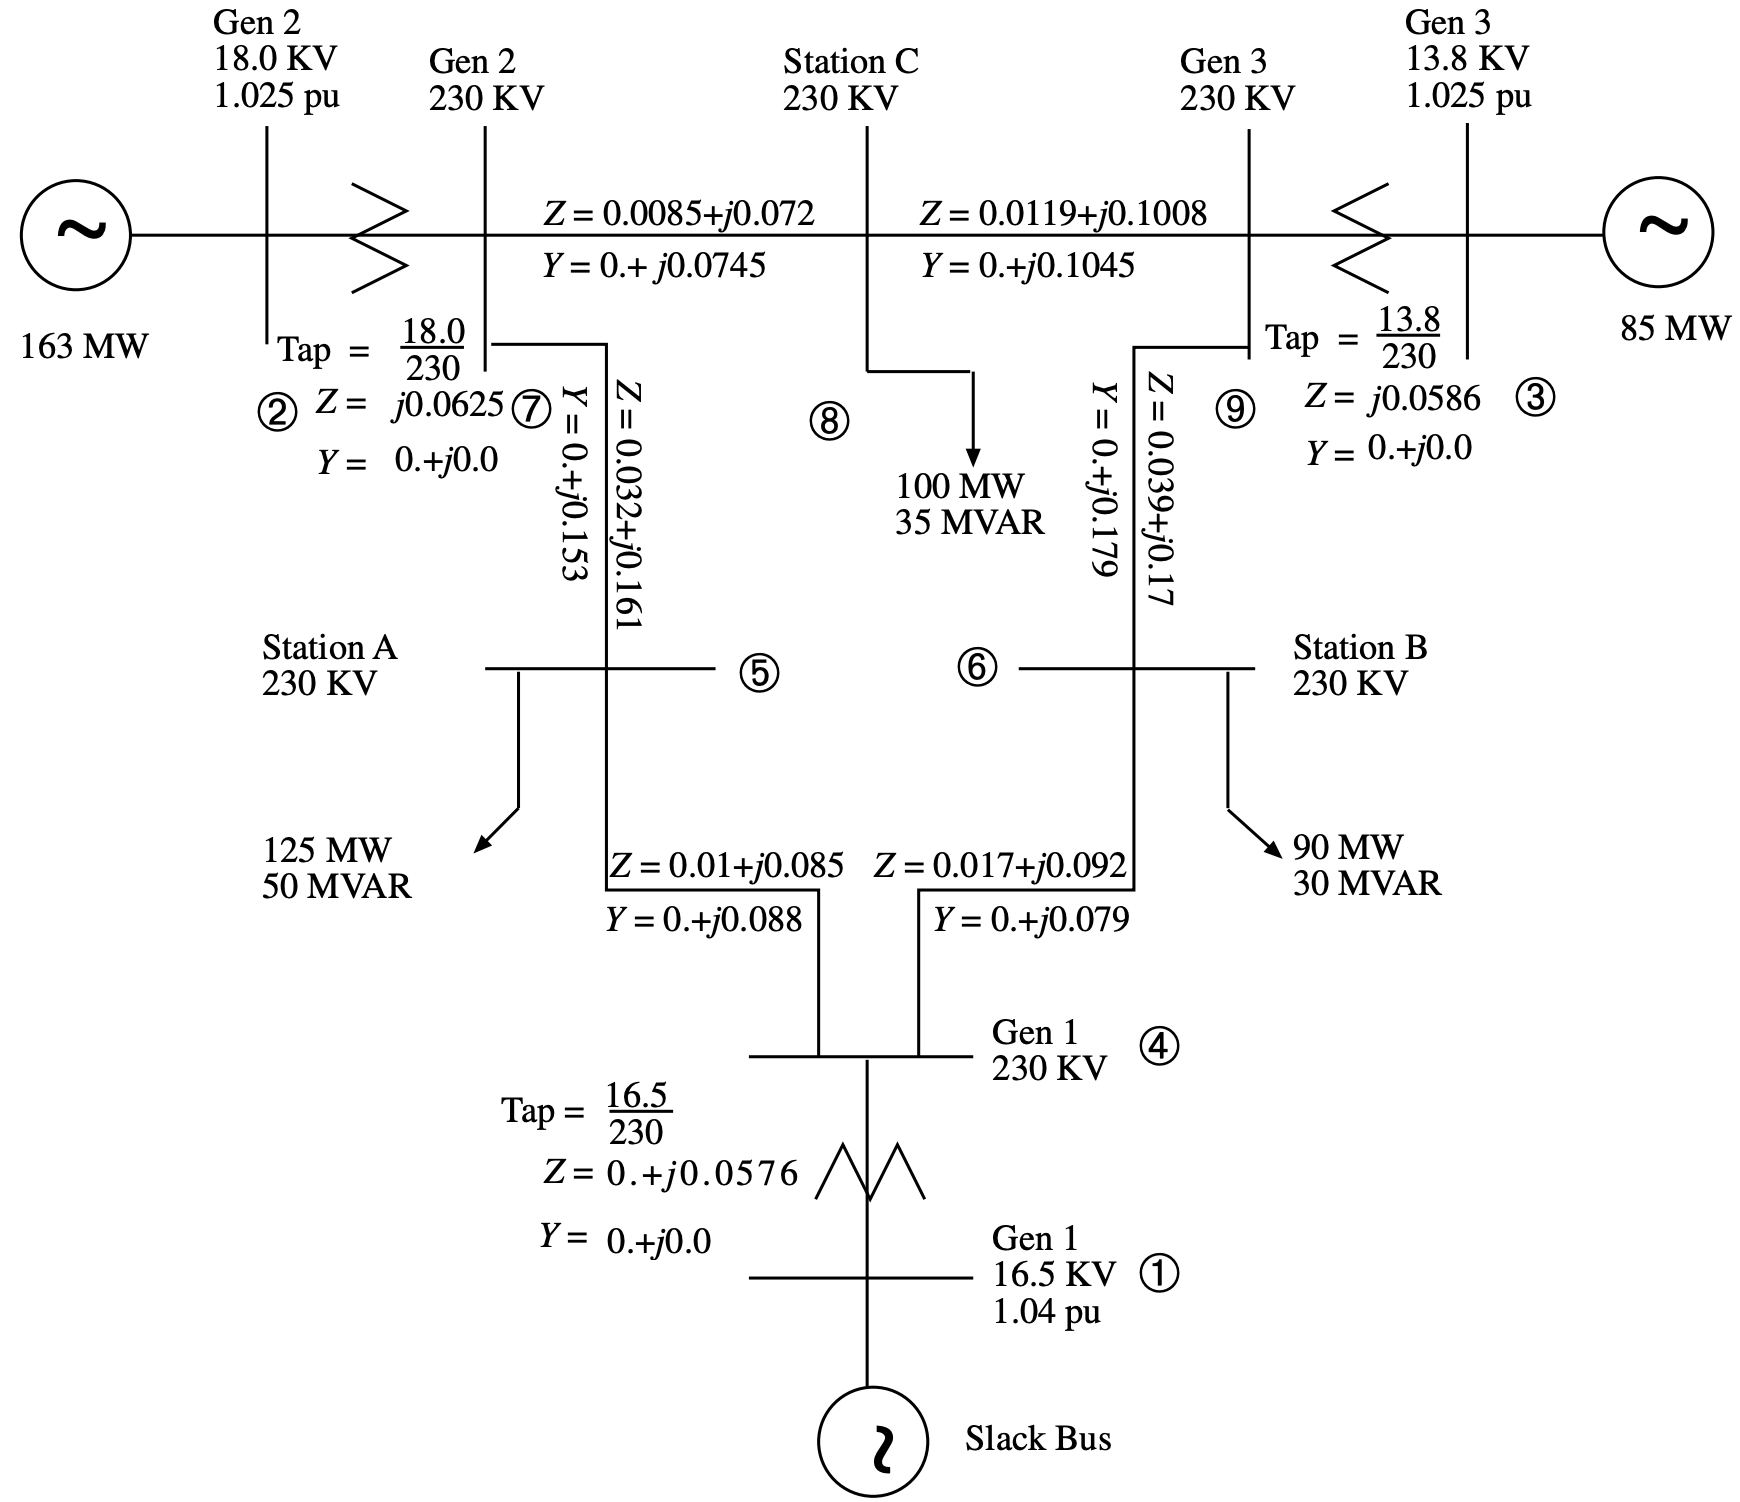
\includegraphics[width = 12cm]{images/WSCC9.png}
    \caption{WECC-9 bus system \cite{sauer2017power}.}
    \label{fig:WSCC9}
\end{figure}

% TODO: mention the saturation function?
In the simulation, the generators are represented by two-axis synchronous
generator (SG) models, and the excitation systems are modeled in accordance with
the IEEE Type-1 specification. Detailed descriptions of these models can be
found in Chapter \ref{chap:vsm-modeling}. The parameters employed in the
simulation are sourced from Sauer and Pai \cite{sauer2017power} and are
conveniently summarized in Tables \ref{tab:gen_params} and \ref{tab:avr_params}
for the reader's reference. Furthermore, we neglect the governors' dynamics and
assume the mechanical power inputs $P_m$ of the generators are constant and
equal to the power flow setpoints. The line admittances and the power flow
setpoints are defined according to Figure \ref{fig:WSCC9}, and the loads are
considered to be of constant power.

\begin{table}[h!]
    \centering
    \begin{tabular}{@{}llll@{}}
        \toprule
        \multicolumn{4}{c}{\textbf{Machine Data}} \\
        \midrule
        Parameters & Generator 1 & Generator 2 & Generator 3 \\
        \midrule
        \( M(\text{secs}^2) \) & 0.125 & 0.034 & 0.016 \\
        \( D(\text{secs}^2) \) & 2 & 2 & 2 \\
        \( X_d(\text{pu}) \) & 0.146 & 0.8958 & 1.3125 \\
        \( X'_d(\text{pu}) \) & 0.0608 & 0.1198 & 0.1813 \\
        \( X_q(\text{pu}) \) & 0.0969 & 0.8645 & 1.2578 \\
        \( X'_q(\text{pu}) \) & 0.0969 & 0.1969 & 0.25 \\
        \( T'_d0(\text{sec}) \) & 8.96 & 6.0 & 5.89 \\
        \( T'_q0(\text{sec}) \) & 0.31 & 0.535 & 0.6 \\
        \bottomrule
    \end{tabular}
    \caption{Synchronous generators' parameters}
    \label{tab:gen_params}
\end{table}
    
\begin{table}[h!]
    \centering
    \begin{tabular}{@{}llll@{}}
    \toprule
    \multicolumn{4}{c}{\textbf{Exciter Data}} \\
    \midrule
    Parameters & Exciter 1 & Exciter 2 & Exciter 3 \\
    \midrule
    \( K_A \) & 20 & 20 & 20 \\
    \( T_A(\text{sec}) \) & 0.2 & 0.2 & 0.2 \\
    \( K_E \) & 1.0 & 1.0 & 1.0 \\
    \( T_E(\text{sec}) \) & 0.314 & 0.314 & 0.314 \\
    \( K_F \) & 0.063 & 0.063 & 0.063 \\
    \( T_F(\text{sec}) \) & 0.35 & 0.35 & 0.35 \\
    \bottomrule
    \end{tabular}
    \caption{Exciters' parameters}
    \label{tab:avr_params}
\end{table}

\section{Simulation scenarios}

The simulations will explore the substitution of the generator at bus 2 with an
ideal two-level, three-phase PWM-VSC, as discussed in Section
\ref{sec:modeling_vsc}.  The rated power and voltage of the converter are
selected to match those of Gen 2, depicted in Figure \ref{fig:WSCC9}. It is
essential to acknowledge that a single converter typically cannot manage such a
high rated power and voltage. In practice, multiple converters would be
connected either in series or in parallel to form a multimodule converter system
\cite{tayyebi2020power, yazdani2010voltage}. For simplicity, this analysis
assumes that a multimodule converter exhibits the same behavior as the ideal
two-level, three-phase PWM-VSC described in Section \ref{sec:modeling_vsc}.
Accordingly, the LCL filter parameters and the voltage and current controller
specifications are detailed in Tables \ref{tab:pwm_vsc_parameters} and
\ref{tab:vsc_controller_parameters} for the reader's convenience.

\begin{table}[h!]
    \centering
    \begin{tabular}{@{}llll@{}}
    \toprule
    \multicolumn{3}{c}{\textbf{PWM-VSC Filter Data}} \\
    \midrule
        Parameter & Value (SI) & Value (pu) \\
        \midrule
        Power rating & 192 MVA & 1 \\
        Rated voltage & 18 kV & 1 \\
        \(L_f\) & 0.5 mH & 0.11 \\
        \(C_f\) & 100 \si{\micro\farad} & 15.71 \\
        \(L_g\) & 0.5 mH & 0.11 \\
    \bottomrule
    \end{tabular}
    \caption{Ideal two-level three phase PWM-VSC filter parameters.}
    \label{tab:pwm_vsc_parameters}
\end{table}

\begin{table}[h!]
    \centering
    \begin{tabular}{@{}llll@{}}
    \toprule
    \multicolumn{2}{c}{\textbf{Controller Data}} \\
    \midrule
        Parameter & Value \\
        \midrule
        \(k_{v,p}\) & 20 \\
        \(k_{v,i}\) & 400 \\
        \(k_{i,p}\) & 2 \\
        \(k_{i,i}\) & 100 \\
    \bottomrule
    \end{tabular}
    \caption{Cascaded voltage and current controller parameters}
    \label{tab:vsc_controller_parameters}
\end{table}

The PI gains for the voltage and current controllers, presented in Table
\ref{tab:vsc_controller_parameters}, were sourced from \cite{du2020comparative}.
The tuning of these controllers is beyond the scope of this thesis. Furthermore,
the parameters for the SG Model block, as shown in Figure
\ref{fig:sm_overall_model}, are identical to those of Generator 2 listed in
Table \ref{tab:gen_params}.

In subsequent sections, four distinct scenarios will be examined:
\begin{itemize}
    \item \textbf{Scenario 1:} All machines depicted in Figure \ref{fig:WSCC9}
    are modeled as 2-axis SGs.
    \item \textbf{Scenario 2:} The SG at bus 2 in Figure \ref{fig:WSCC9} is
    replaced with a CVSM converter, utilizing the classical SG model within the
    SG Model block (Figure \ref{fig:sm_overall_model}).
    \item \textbf{Scenario 3:} The SG at bus 2 in Figure \ref{fig:WSCC9} is
    substituted with a CVSM converter, employing a 1-axis SG model within the SG
    Model block (Figure \ref{fig:sm_overall_model}).
    \item \textbf{Scenario 4:} The SG at bus 2 in Figure \ref{fig:WSCC9} is
    supplanted by a CVSM converter, using a 2-axis SG model in the SG Model
    block (Figure \ref{fig:sm_overall_model}).
\end{itemize}

\section{Simulation of Load Increase} \label{sec:load_increase}
In this section, we examine the system's transient response to a 10\% step
increase in active power demand at bus 8, illustrated in Figure \ref{fig:WSCC9}.
The selection of bus 8 for introducing the disturbance is strategic, owing to
its close proximity to bus 2—the site of the Converter-Based Synchronous Machine
(CVSM). This proximity allows for an in-depth analysis of the CVSM's dynamic
impact on neighboring buses under conditions of substantial load changes.

The load increase is modeled as a step signal, starting at $t=1s$ and lastig
until the end of the simulation at $t=10s$. The transient response of the
frequency, voltage, current and active and reactive powers at the generator
buses are then evaluated to understand how the CVSM behaves compared to a SG,
and how it affects the dynamics of the other generators in the same area.

As illustrated in Figures \ref{fig:omega_load_increase},
\ref{fig:voltage_load_increase},\ref{fig:current_load_increase},\ref{fig:active_load_increase}
and \ref{fig:reactive_load_increase} the scenarios 1 and 4 present virtually a
perfect fit, meaning that the developed CVSM can can precisely replicate the
behavior of a 2-axis SG when its model is employed in the SG Model block
depicted in Figure \ref{fig:generic_gfmi}. Scenarios 3 and 4 demonstrate very
akin responses, with minor discrepancies observable only in voltage magnitude
and reactive power. These negligible differences, however, do not signify
inferior performance. 

Conversely, Scenario 2 exhibits a markedly different response across all
parameters. Although the CVSM configured with a classical model exhibits
improved inertia and damping properties, the transient response of generators at
Buses 1 and 3 is adversely affected. Despite the system remaining stable and
eventually settling at the same steady-state values as the other scenarios, it
experiences significantly larger oscillations. These pronounced peaks have the
potential to harm the converter or trigger protective mechanisms.

\newpage
\begin{figure}[ht!]
    \centering
    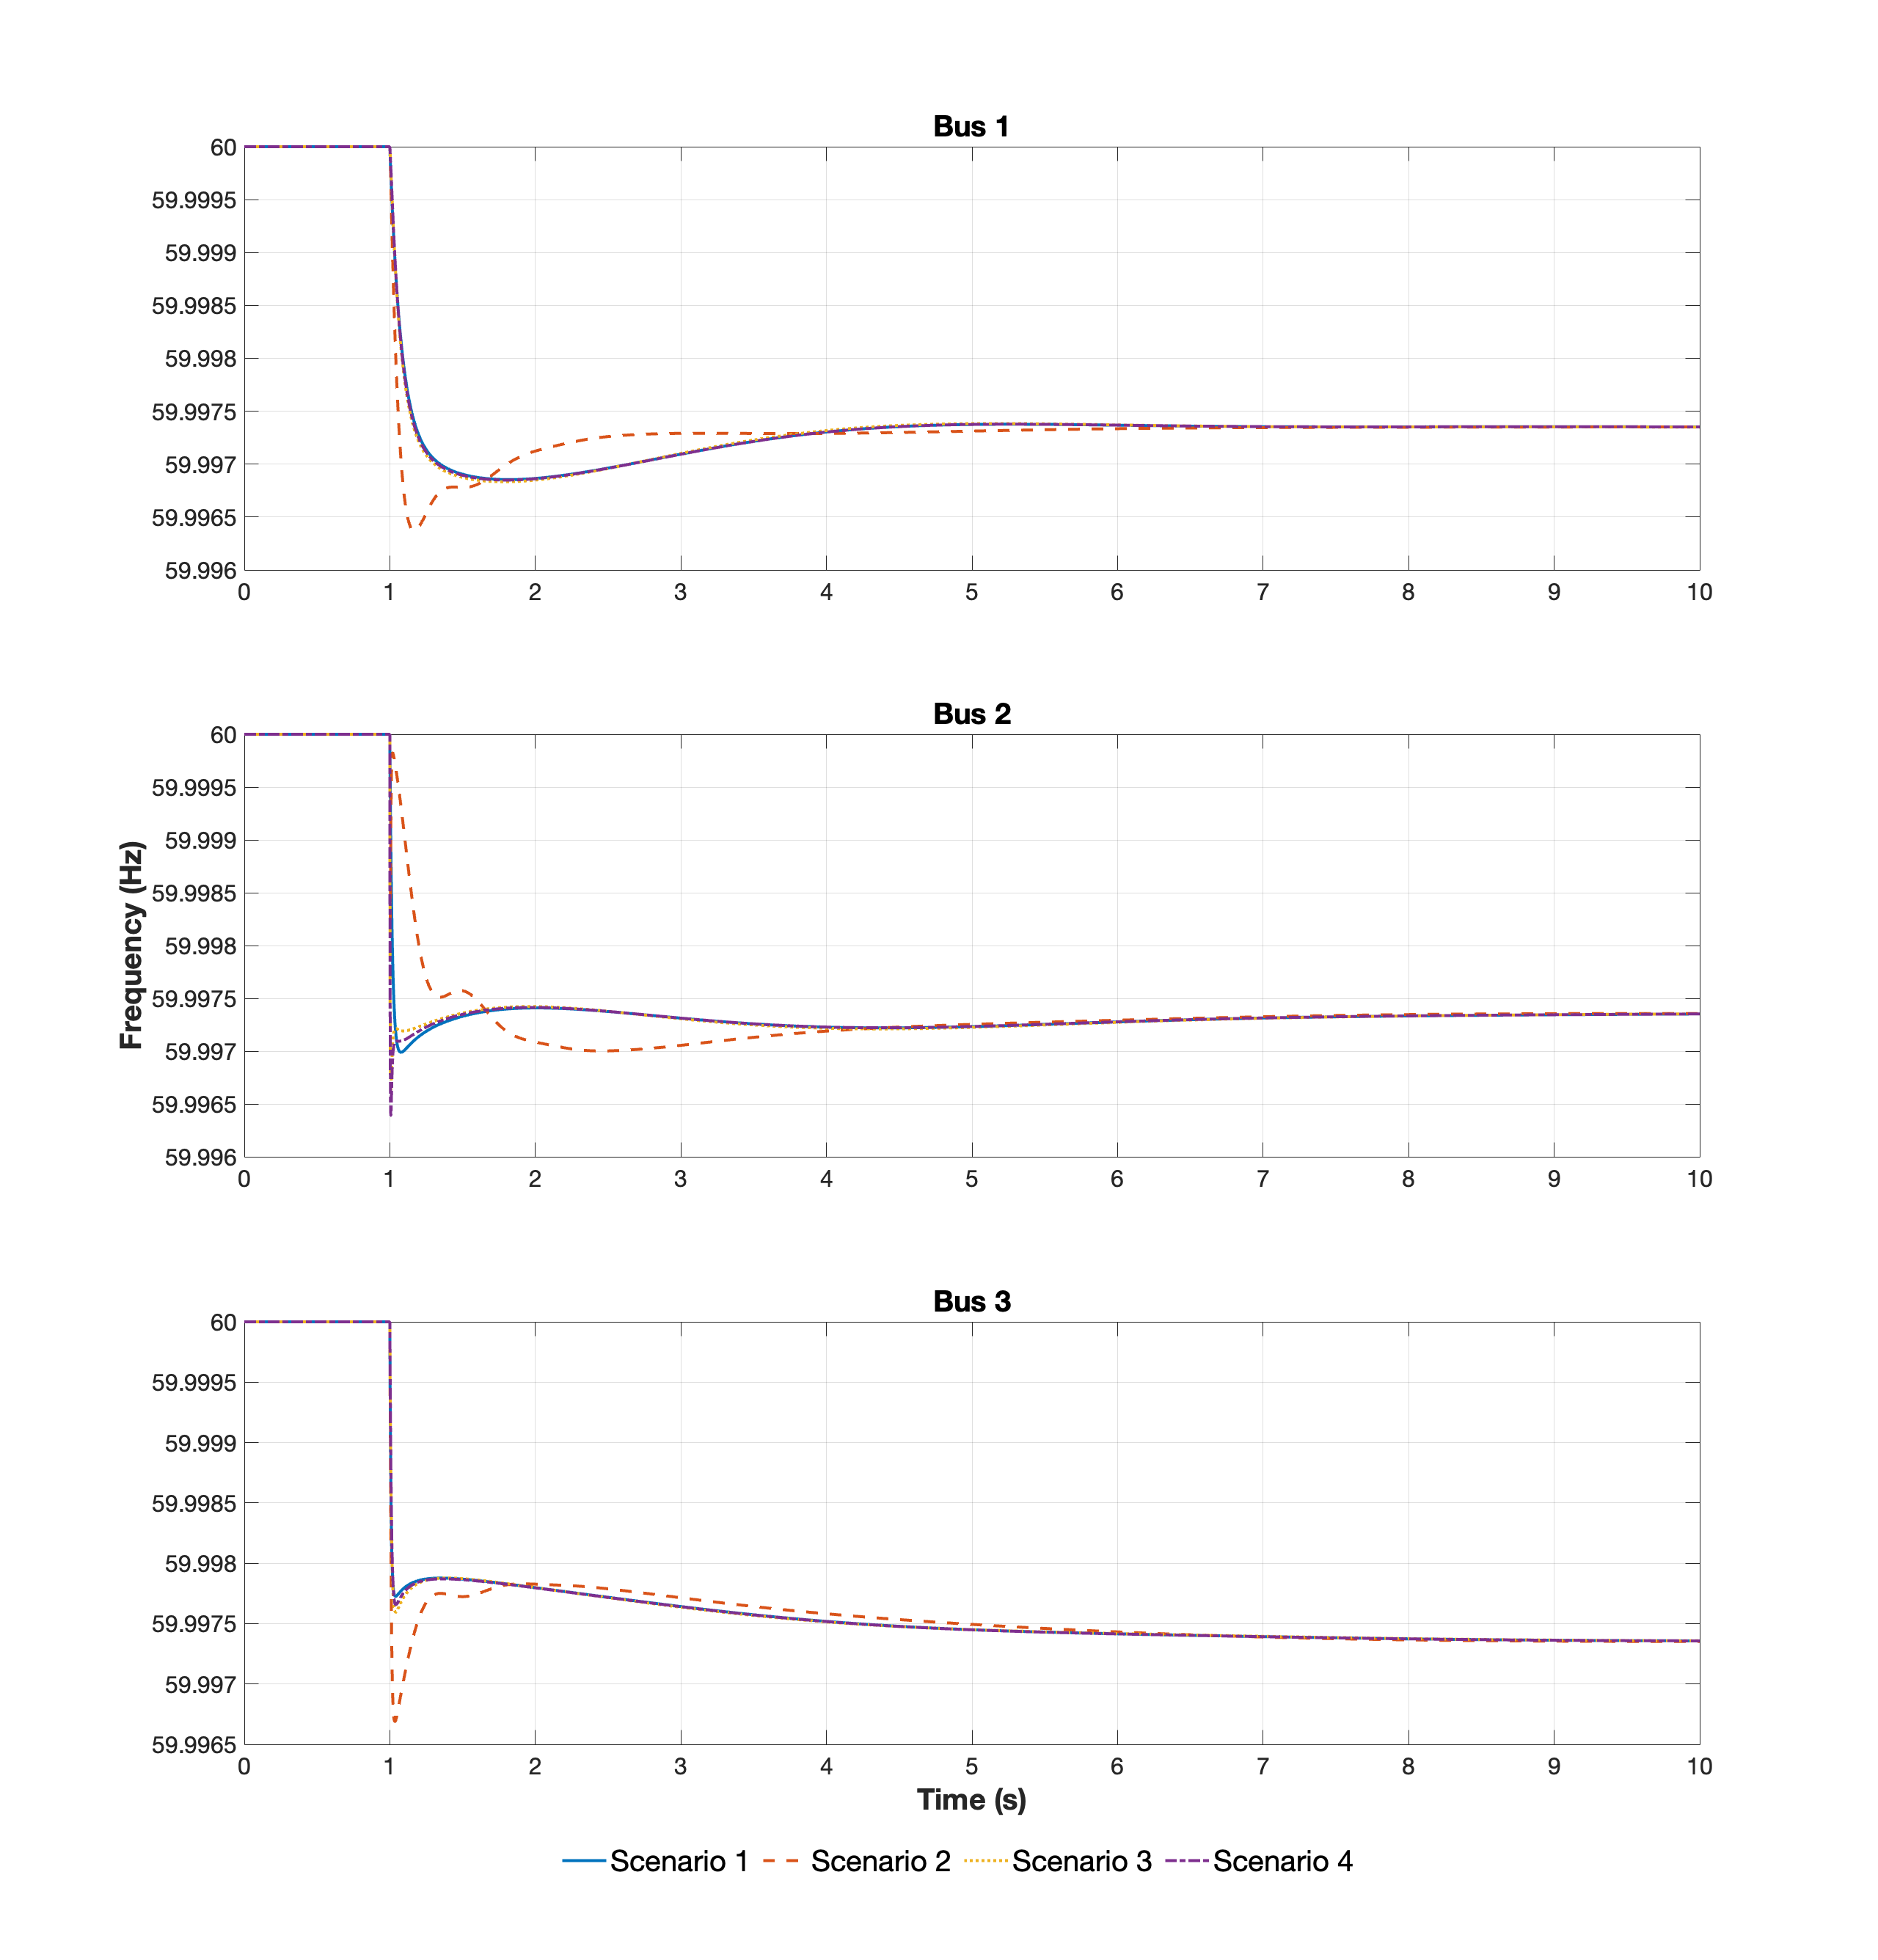
\includegraphics[width = \linewidth]{images/omega_load_increase.png}
    \caption{Transient reponse to load increase of the frequency in the generator buses of the four scenarios.}
    \label{fig:omega_load_increase}
\end{figure}

\newpage
\begin{figure}[ht!]
    \centering
    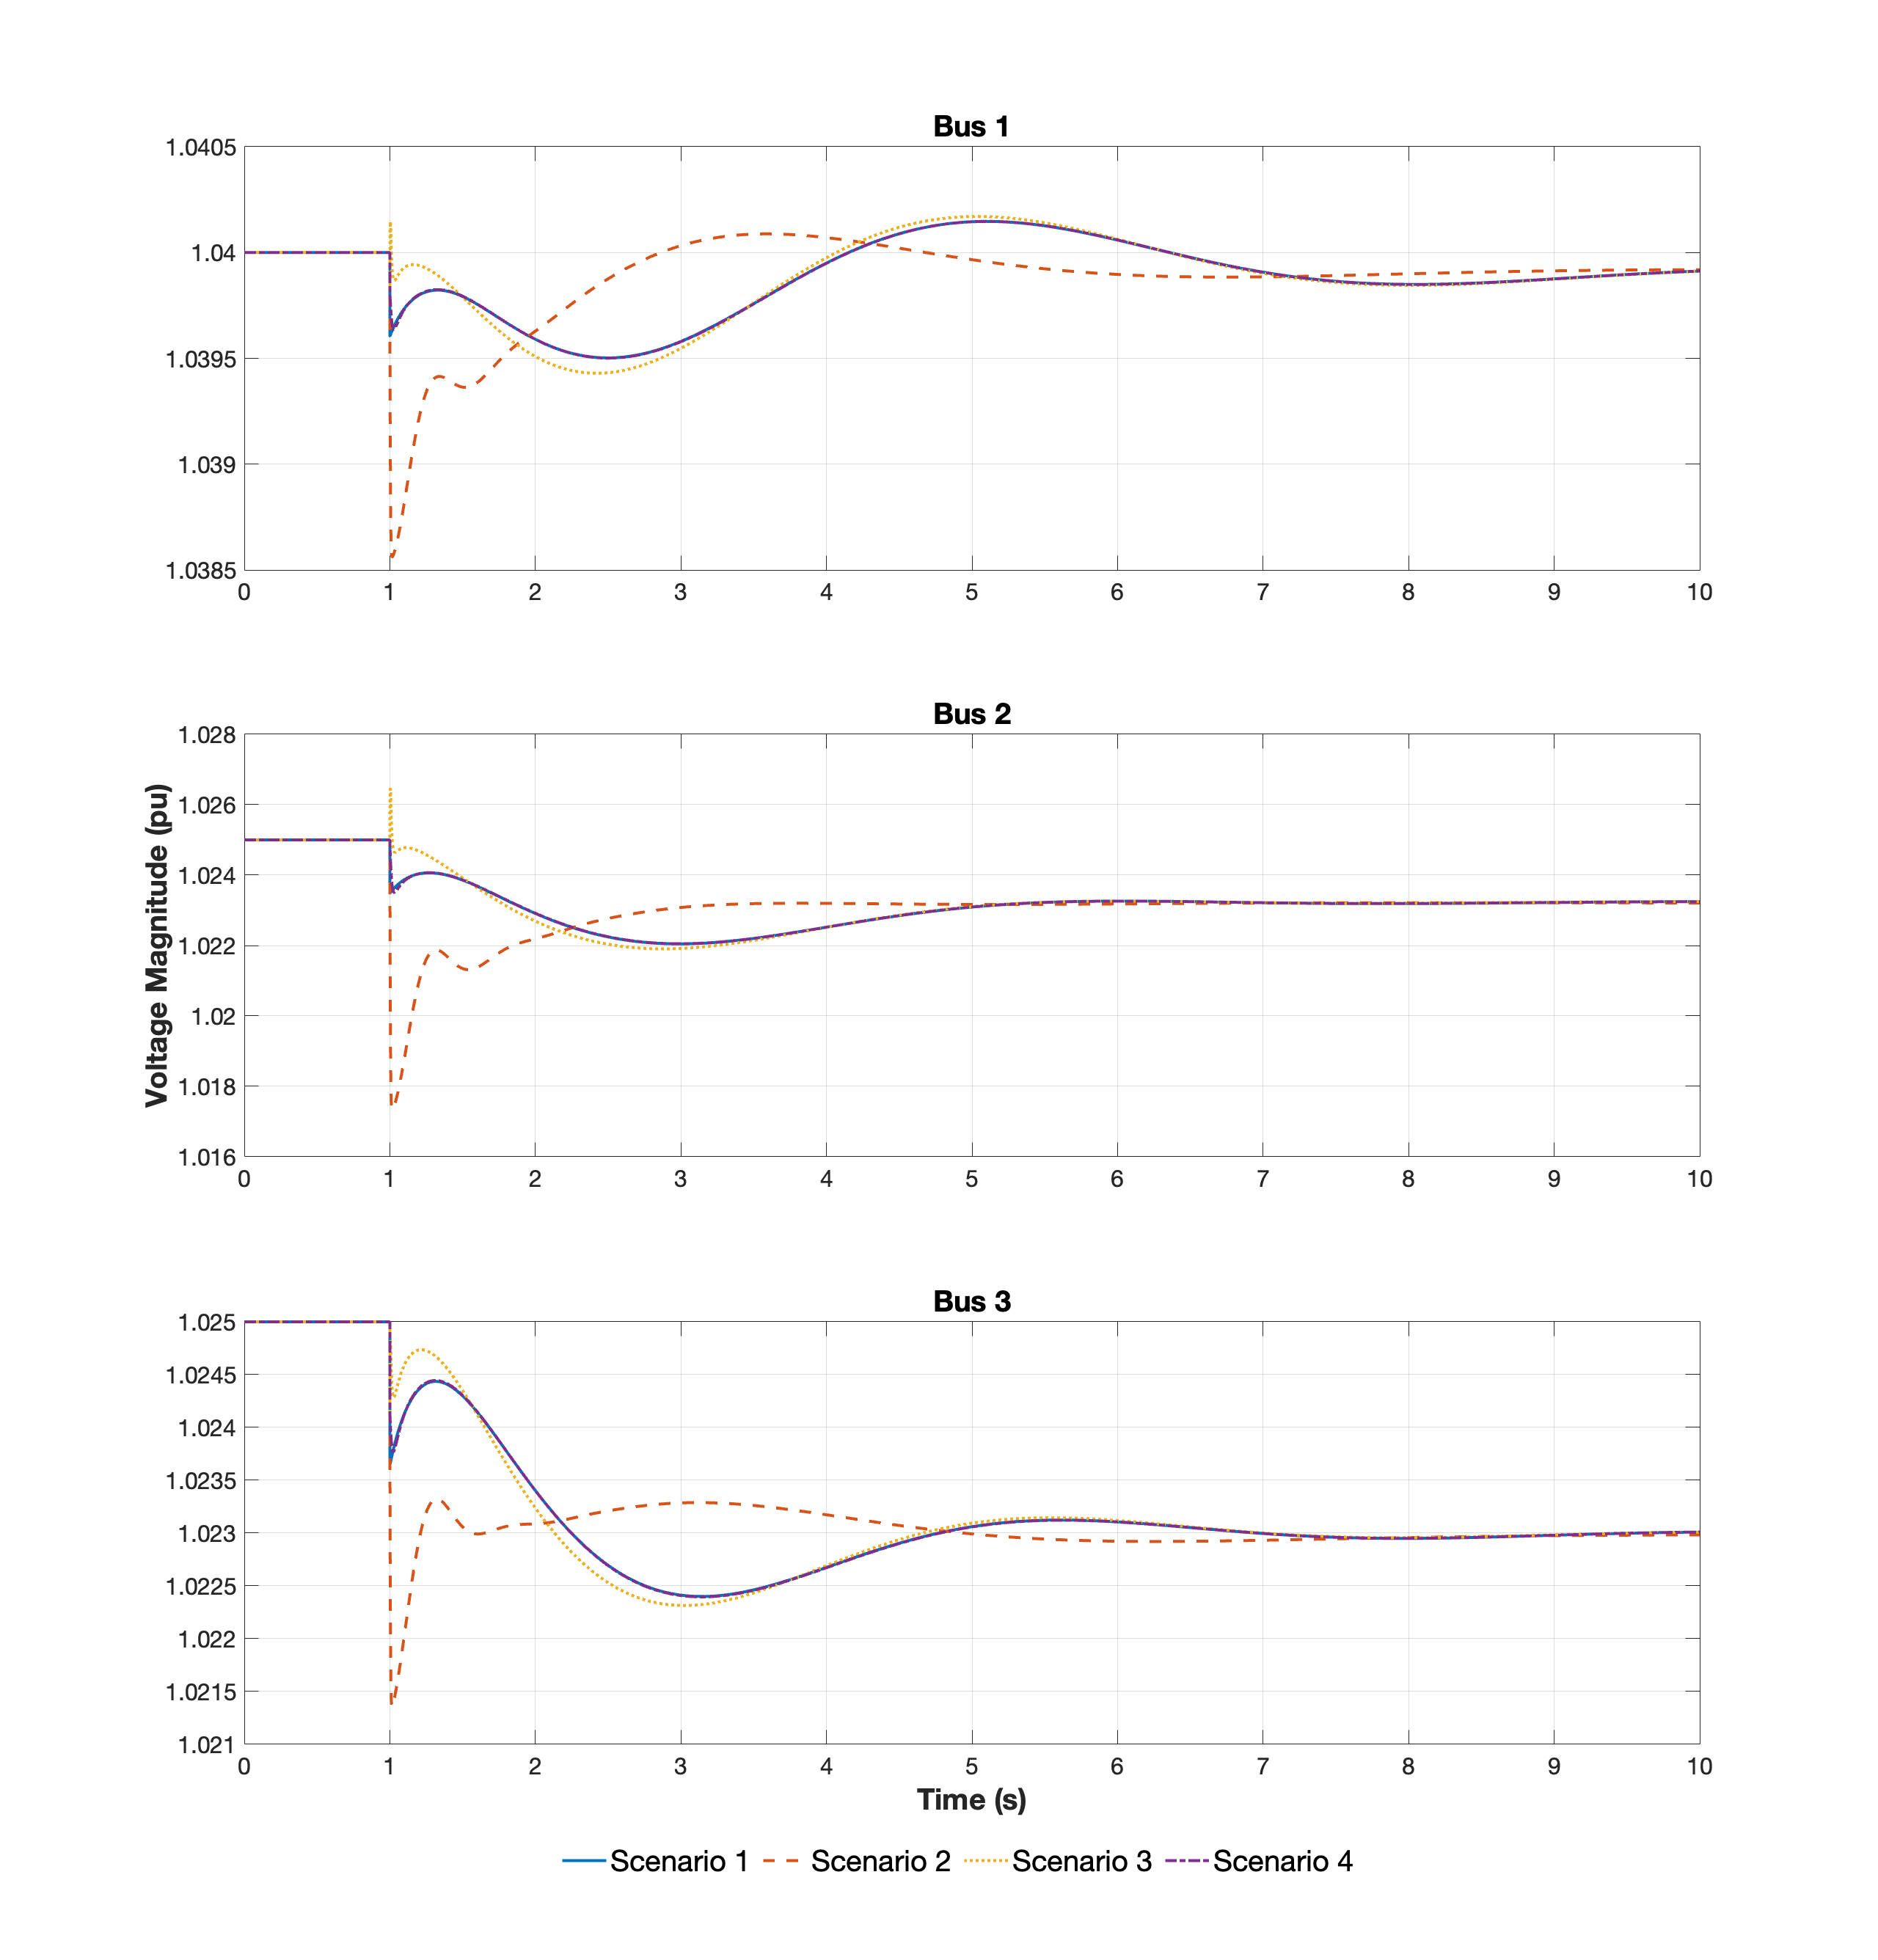
\includegraphics[width = \linewidth]{images/voltage_load_increase.png}
    \caption{Transient reponse to load increase: voltage magnitude in the generator buses of the four scenarios.}
    \label{fig:voltage_load_increase}
\end{figure}

\newpage
\begin{figure}[ht!]
    \centering
    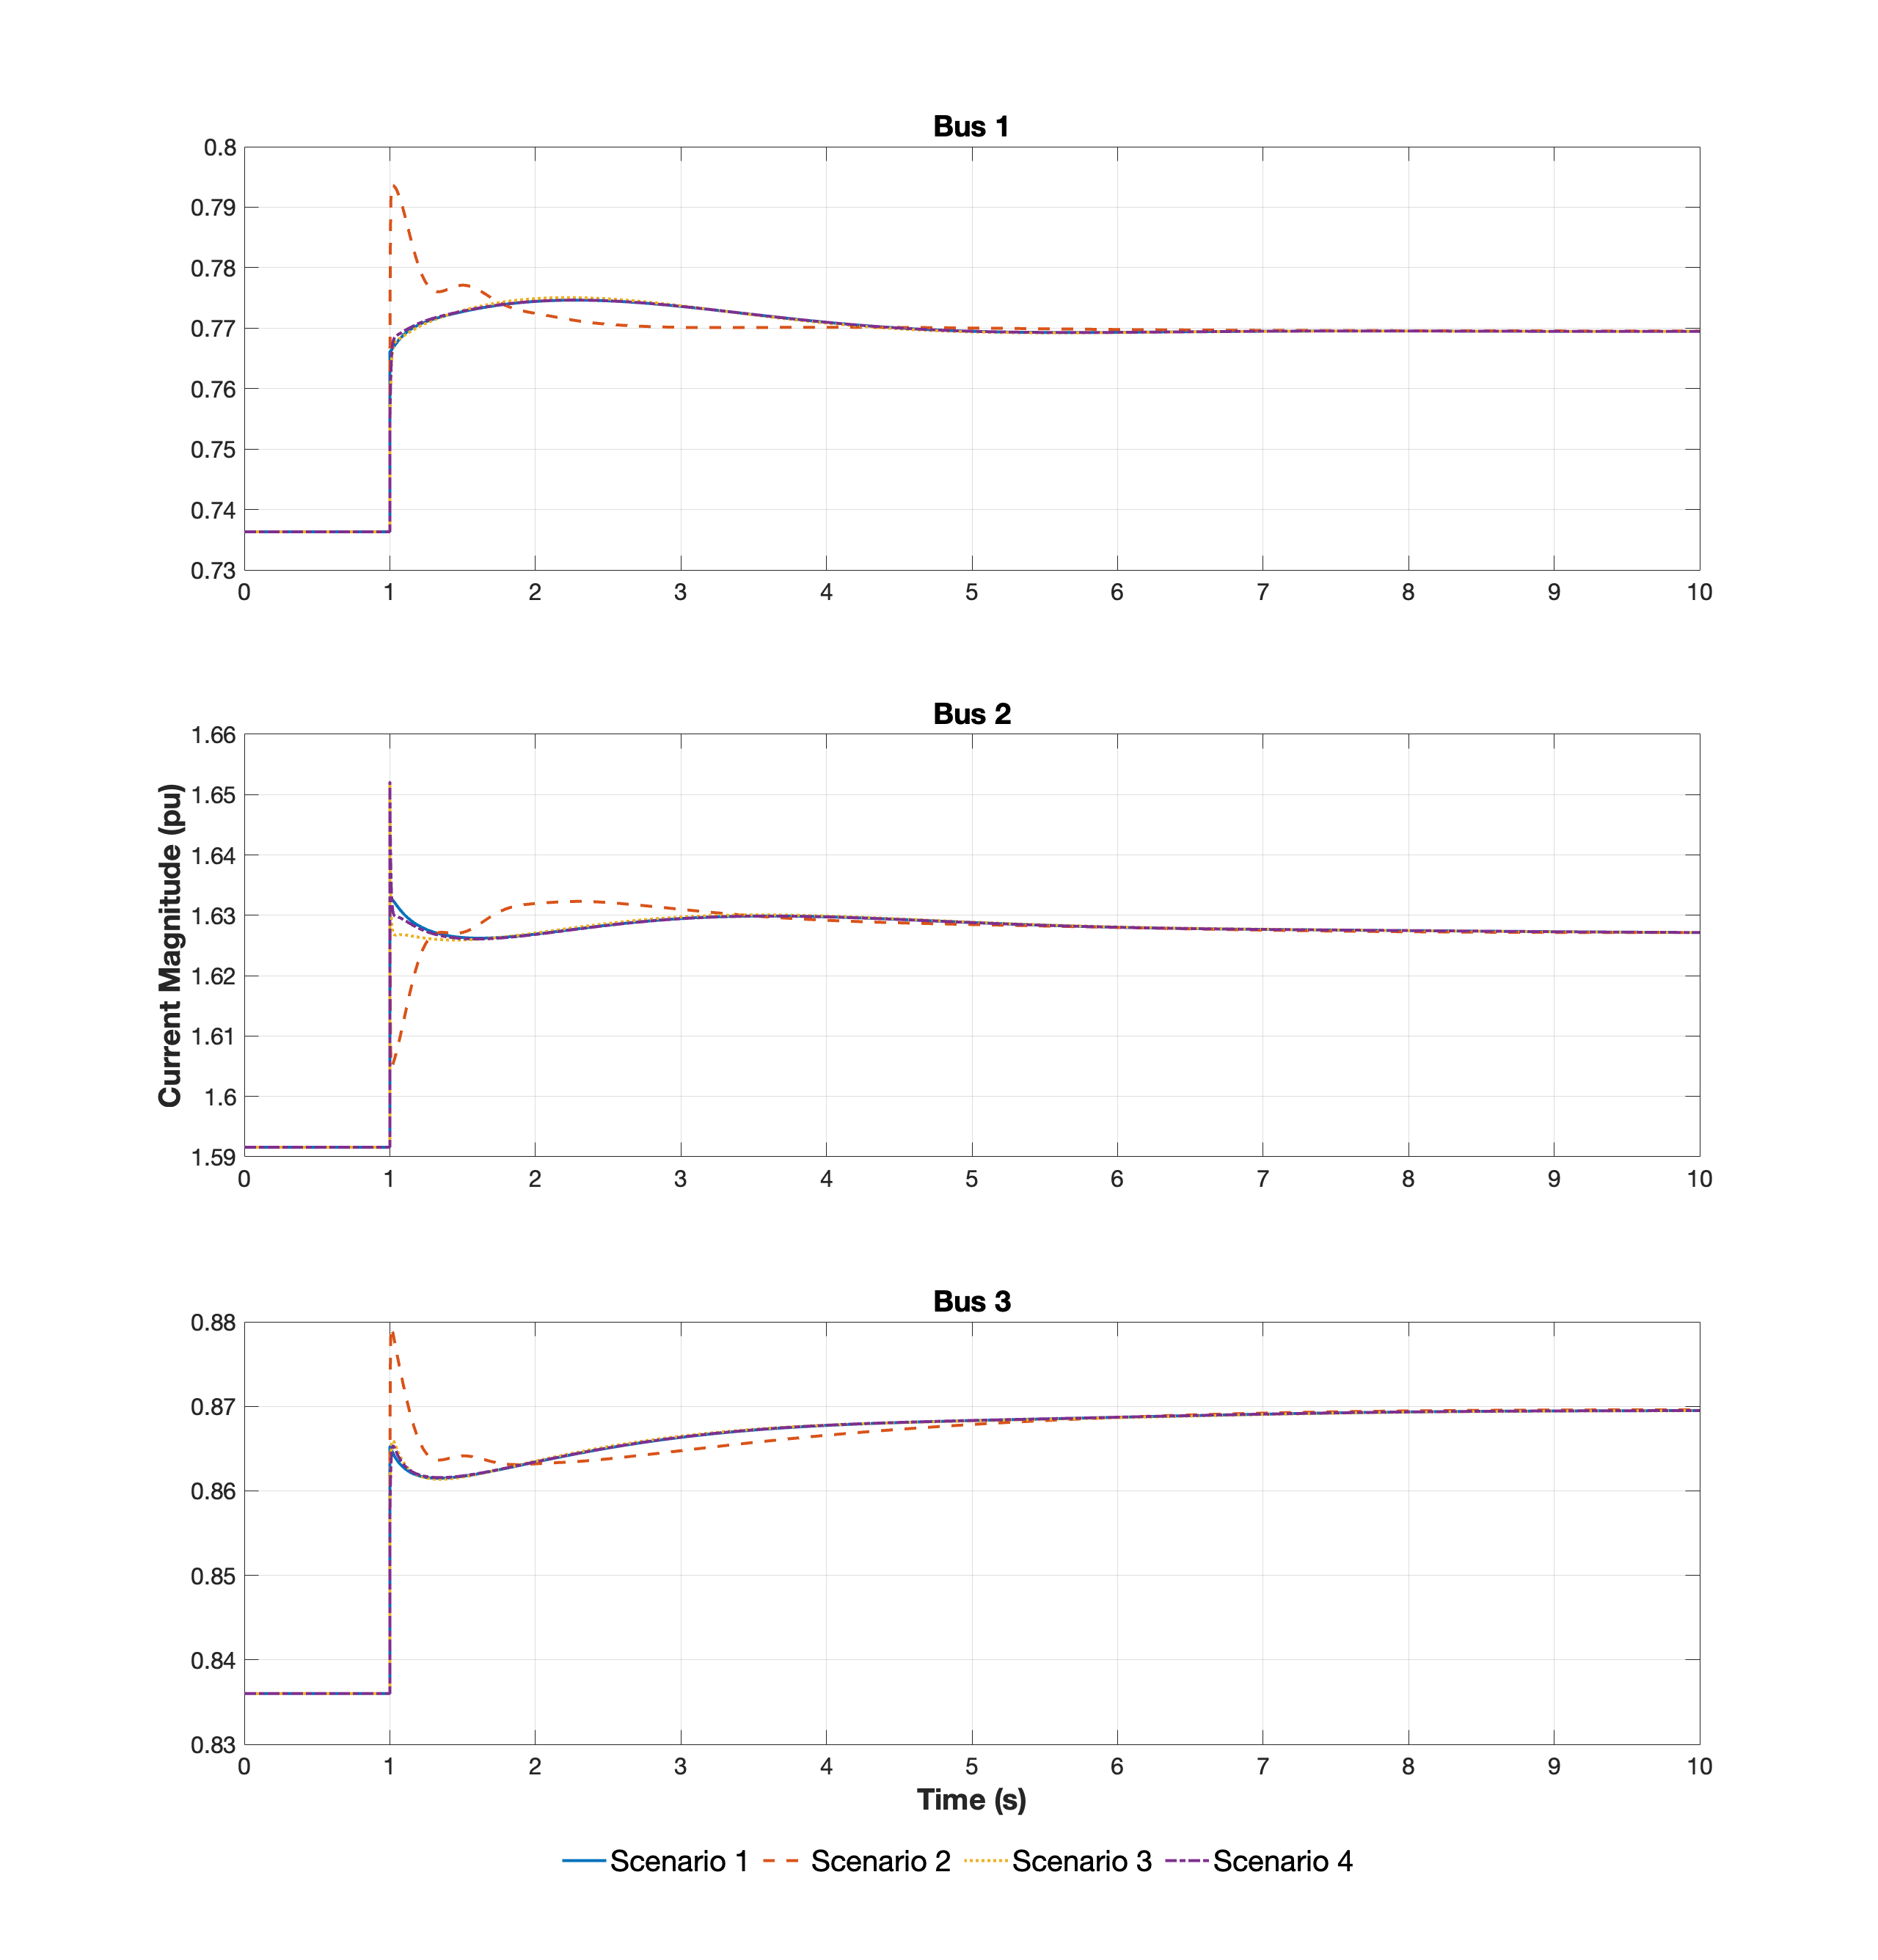
\includegraphics[width = \linewidth]{images/current_load_increase.png}
    \caption{Transient reponse to load increase: current magnitude in the generator buses of the four scenarios.}
    \label{fig:current_load_increase}
\end{figure}

\newpage
\begin{figure}[ht!]
    \centering
    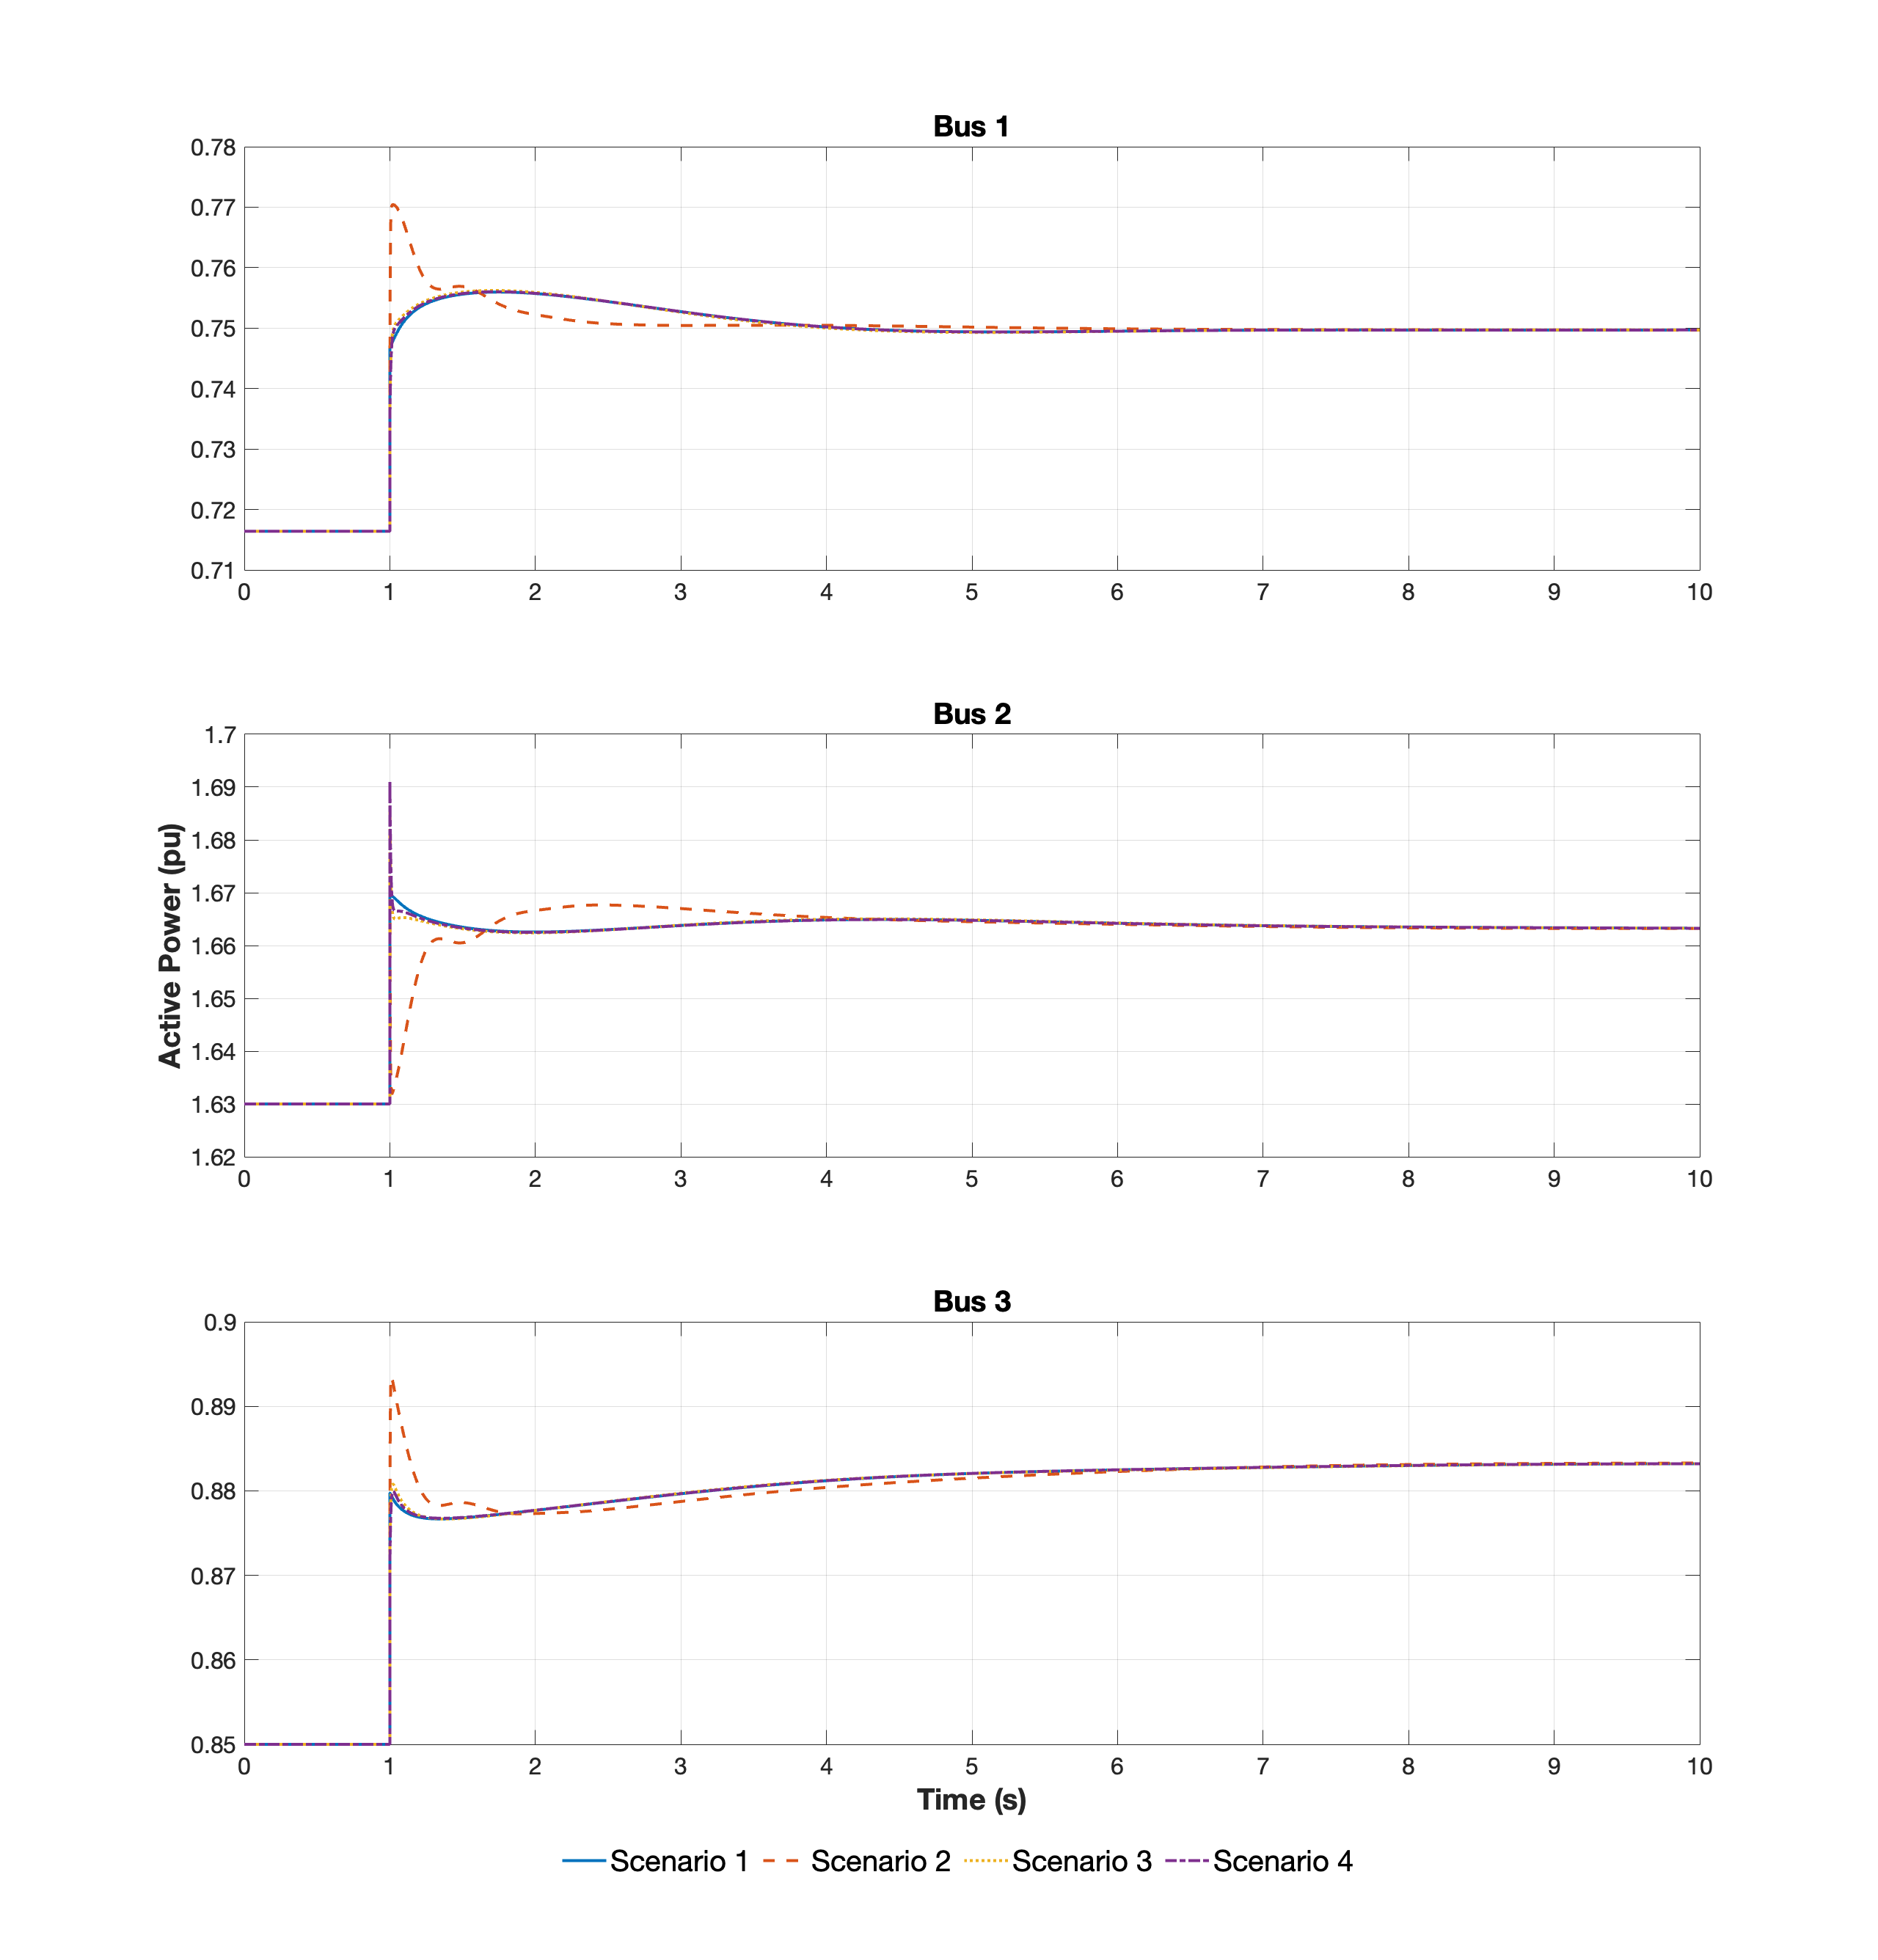
\includegraphics[width = \linewidth]{images/active_load_increase.png}
    \caption{Transient reponse to load increase: active power in the generator buses of the four scenarios.}
    \label{fig:active_load_increase}
\end{figure}

\newpage
\begin{figure}[ht!]
    \centering
    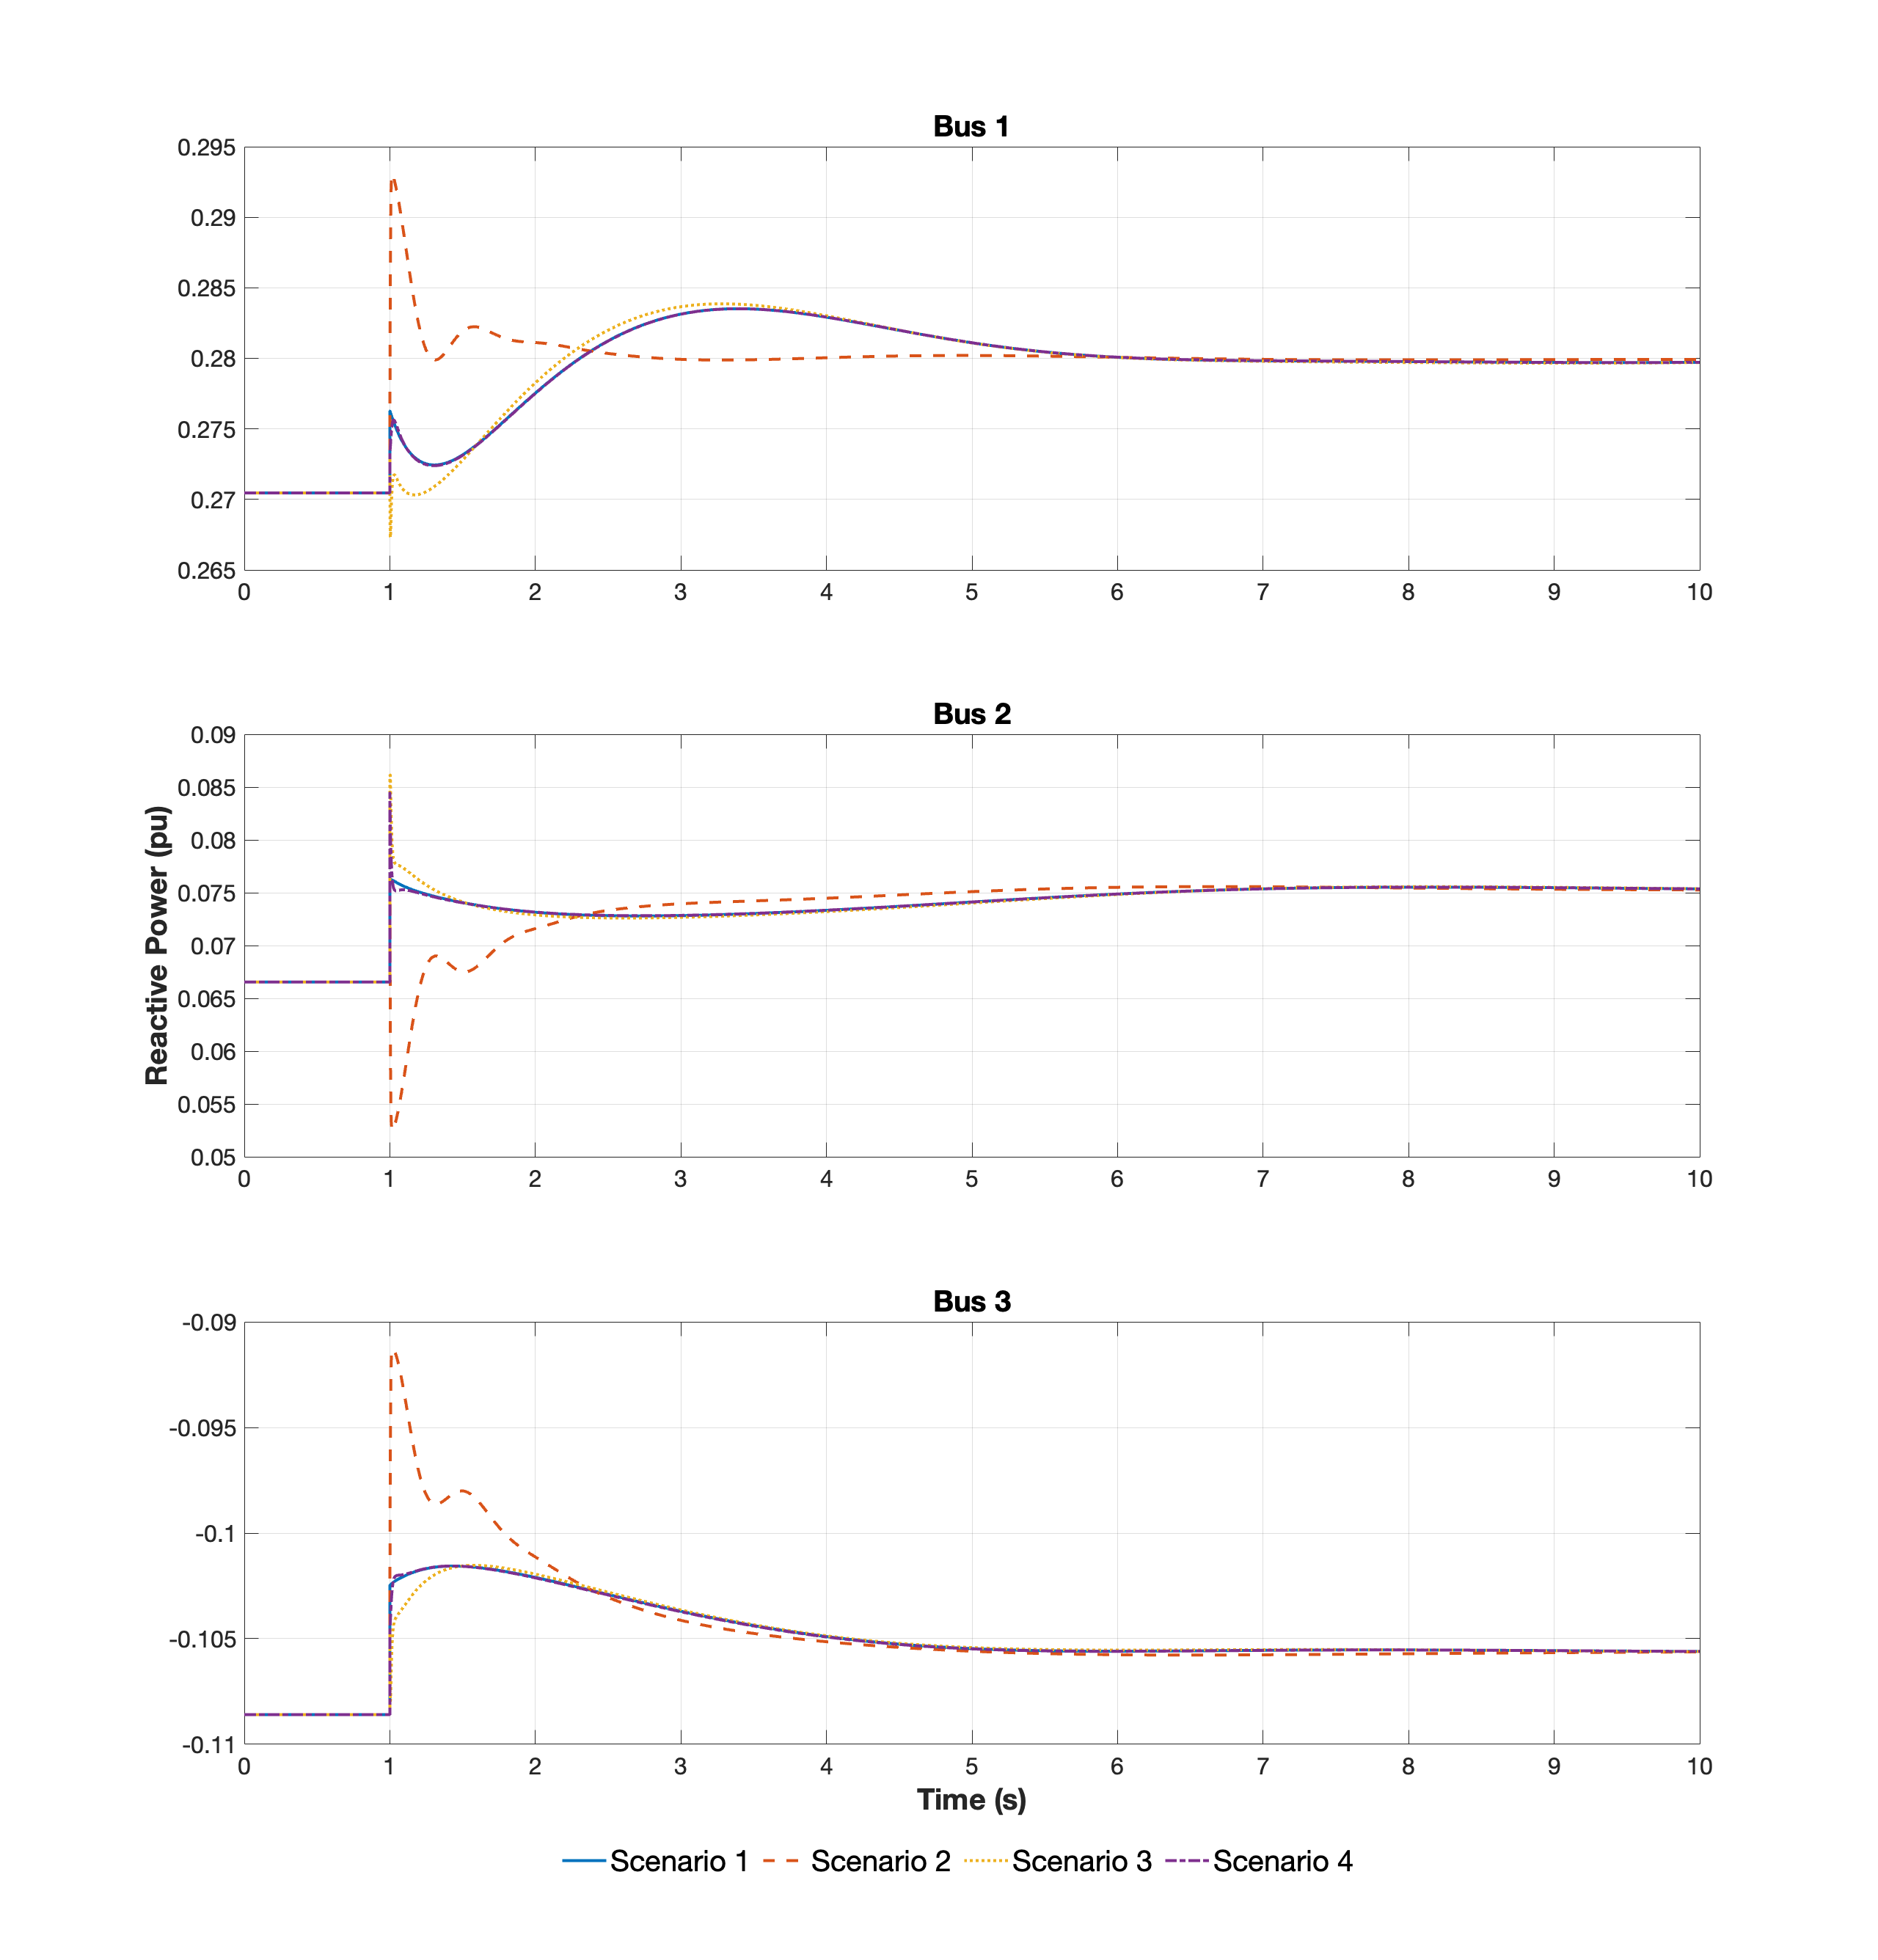
\includegraphics[width = \linewidth]{images/reactive_load_increase.png}
    \caption{Transient reponse to load increase: reactive power in the generator buses of the four scenarios.}
    \label{fig:reactive_load_increase}
\end{figure}

\section{Simulation of Disconnection}\label{sec:disconnection}

In this section, we explore the effects of bus disconnection on the system
dynamics by simulating the complete isolation of bus 8 from the grid. This
disconnection event is modeled as an abrupt step change that reduces the active
and reactive power consumption at bus 8 to zero. The primary aim of this
simulation is to assess the response of the CVSM with both 1-axis and 2-axis
models during a significant disturbance, and to benchmark their performance
against a conventional 2-axis synchronous generator (referred to as Scenario 1).

Figures \ref{fig:omega_disconnection}, \ref{fig:voltage_disconnection},
\ref{fig:current_disconnection}, \ref{fig:active_disconnection} and
\ref{fig:reactive_disconnection} illustrate the transient response of Scenarios
1,3 and 4 to a disconnection at $t=1s$ that lasts until the end of the simulation
at $t=10s$. It's noteworthy that Scenario 2 is excluded from the simulation due
to the classical model of the CVSM's inability to maintain stability under
severe disturbances, highlighting a significant limitation of this approach.

The simulation results clearly demonstrate that the CVSM configurations, both
with 1-axis and 2-axis models, exhibit robust performance that is on par with
that of the traditional 2-axis synchronous generator, even in the face of
substantial disturbances. Given the negligible differences between the 1-axis
and 2-axis CVSM models in handling large disturbances, the subsequent section
will delve into the impact of virtual transient reactance. This analysis will
facilitate a more informed decision on the necessity of the more complex 2-axis
CVSM model versus the sufficiency of the simpler 1-axis model for emulating
synchronous generator behavior in grid-forming applications.

\begin{figure}[ht!]
    \centering
    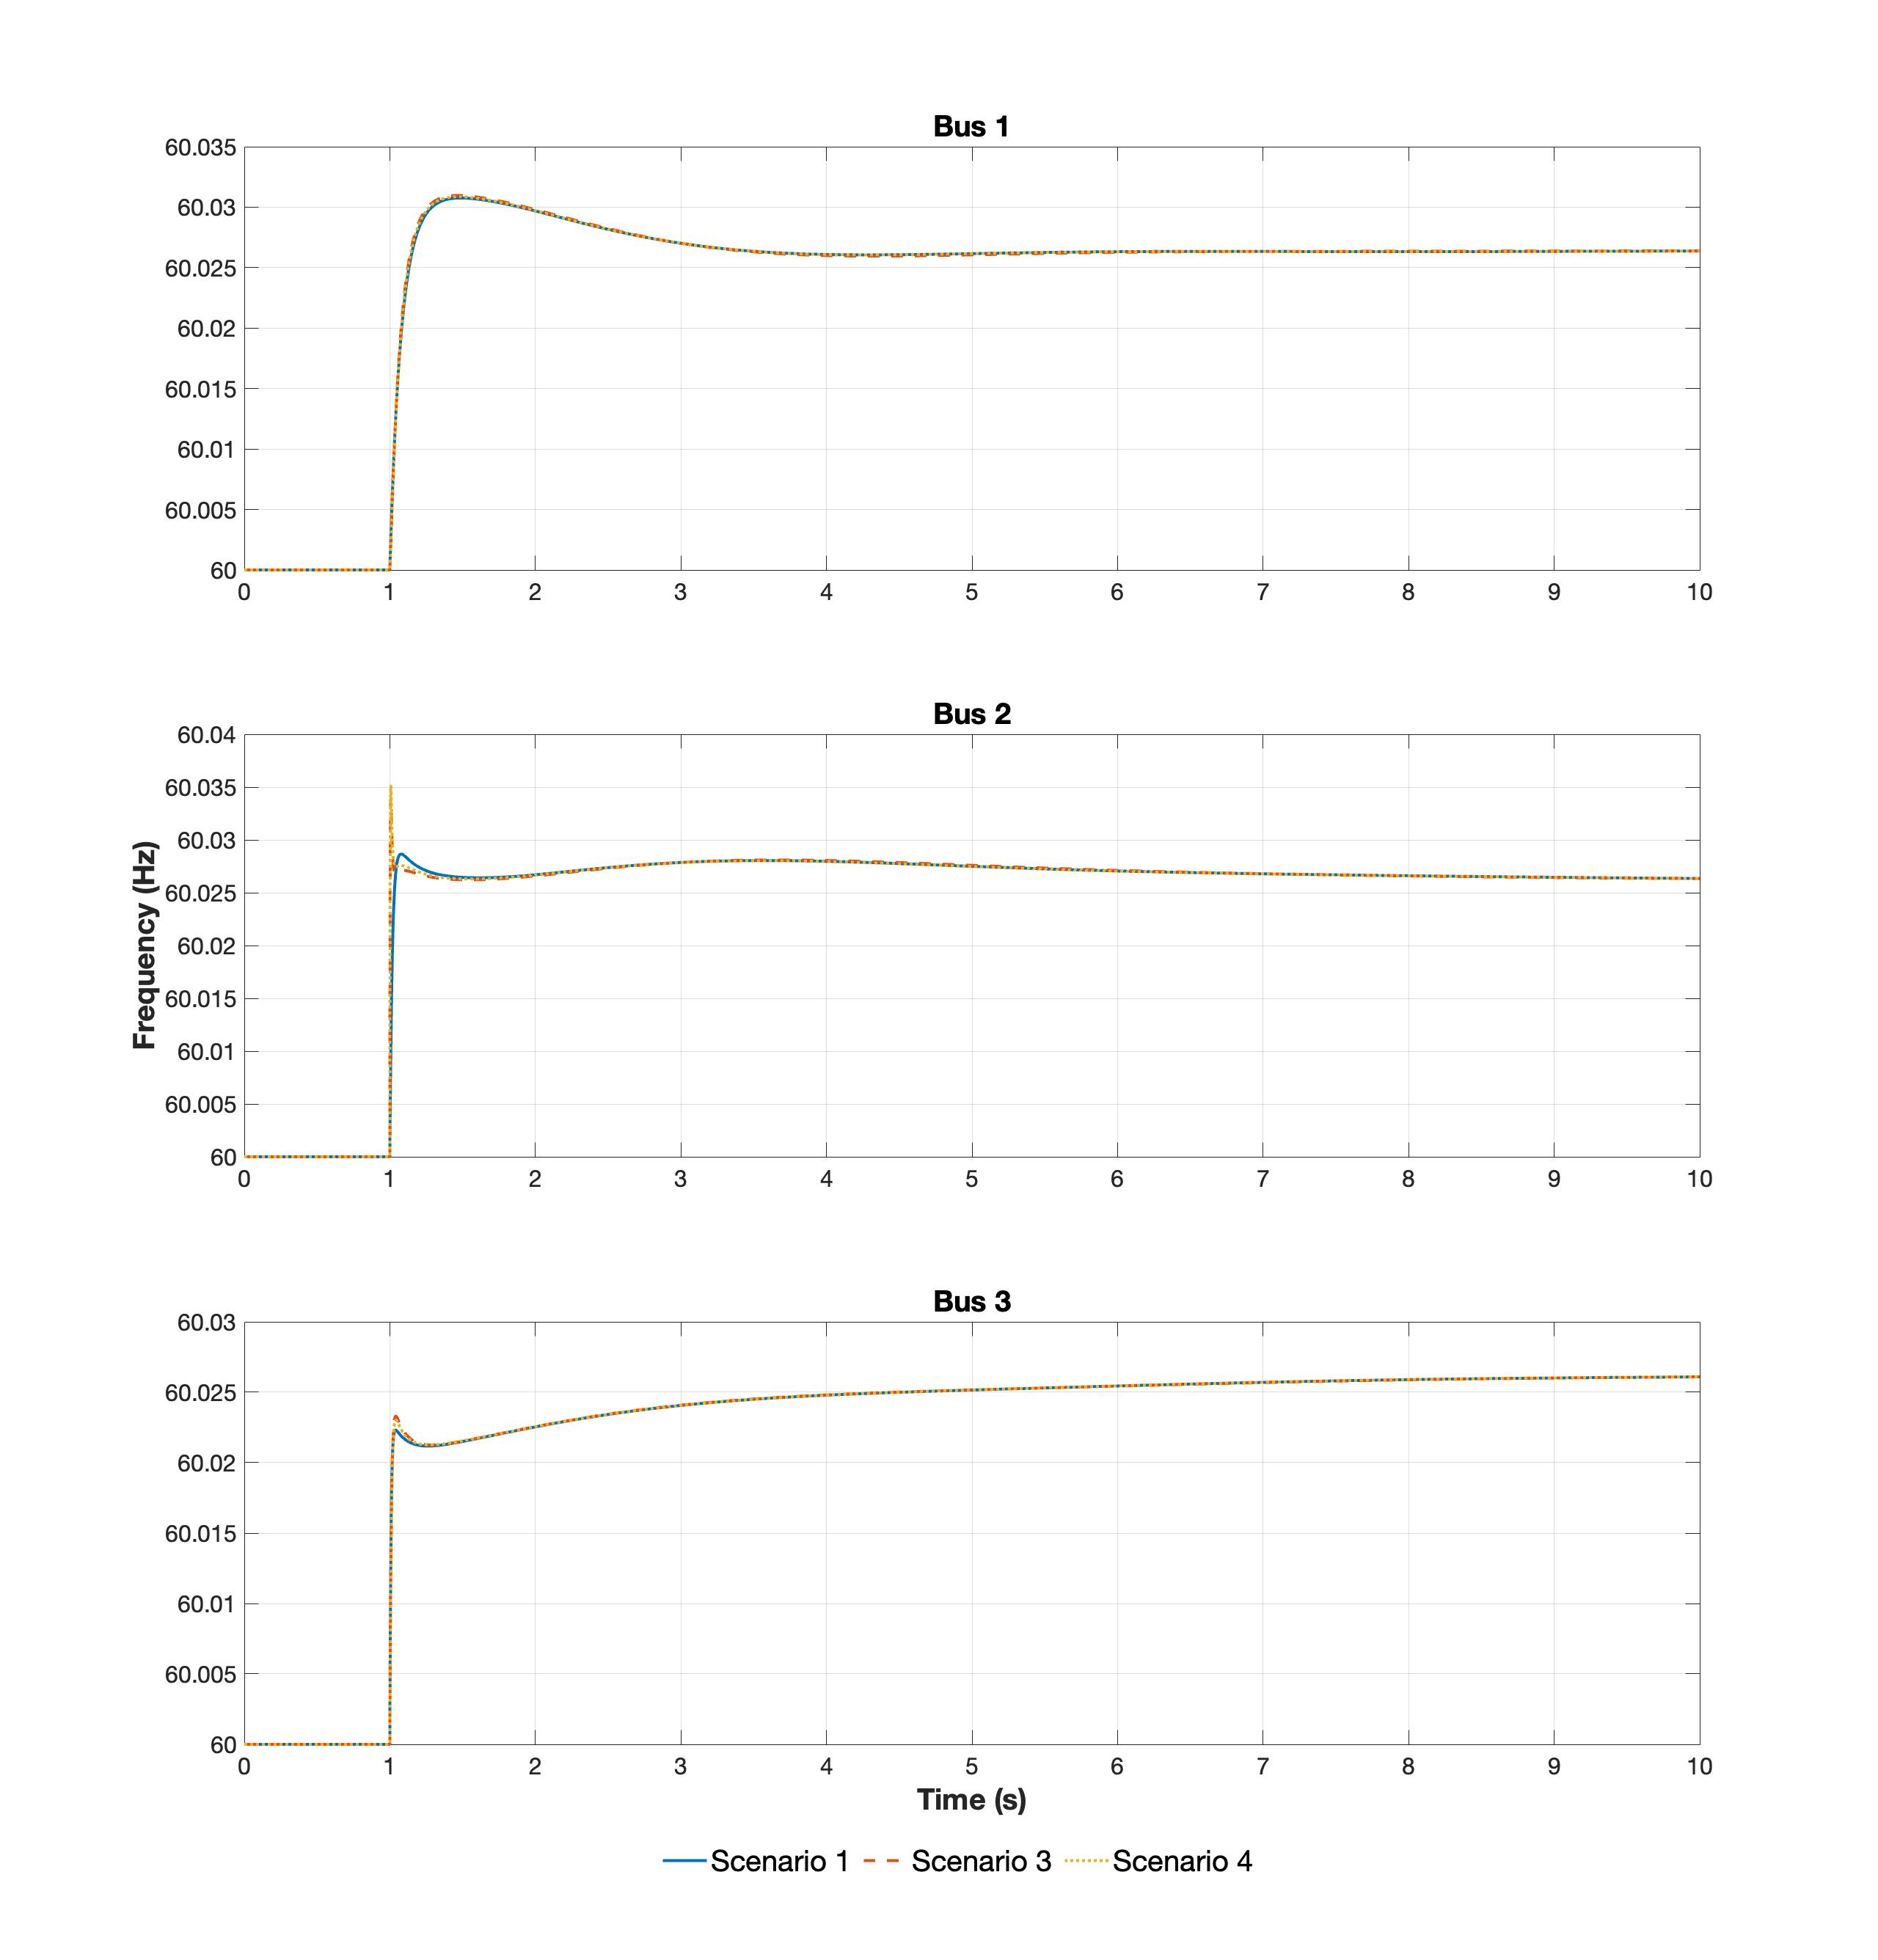
\includegraphics[width = \linewidth]{images/omega_disconnection.png}
    \caption{Transient reponse to disconnection: frequency in the generator buses of the four scenarios.}
    \label{fig:omega_disconnection}
\end{figure}

\newpage
\begin{figure}[ht!]
    \centering
    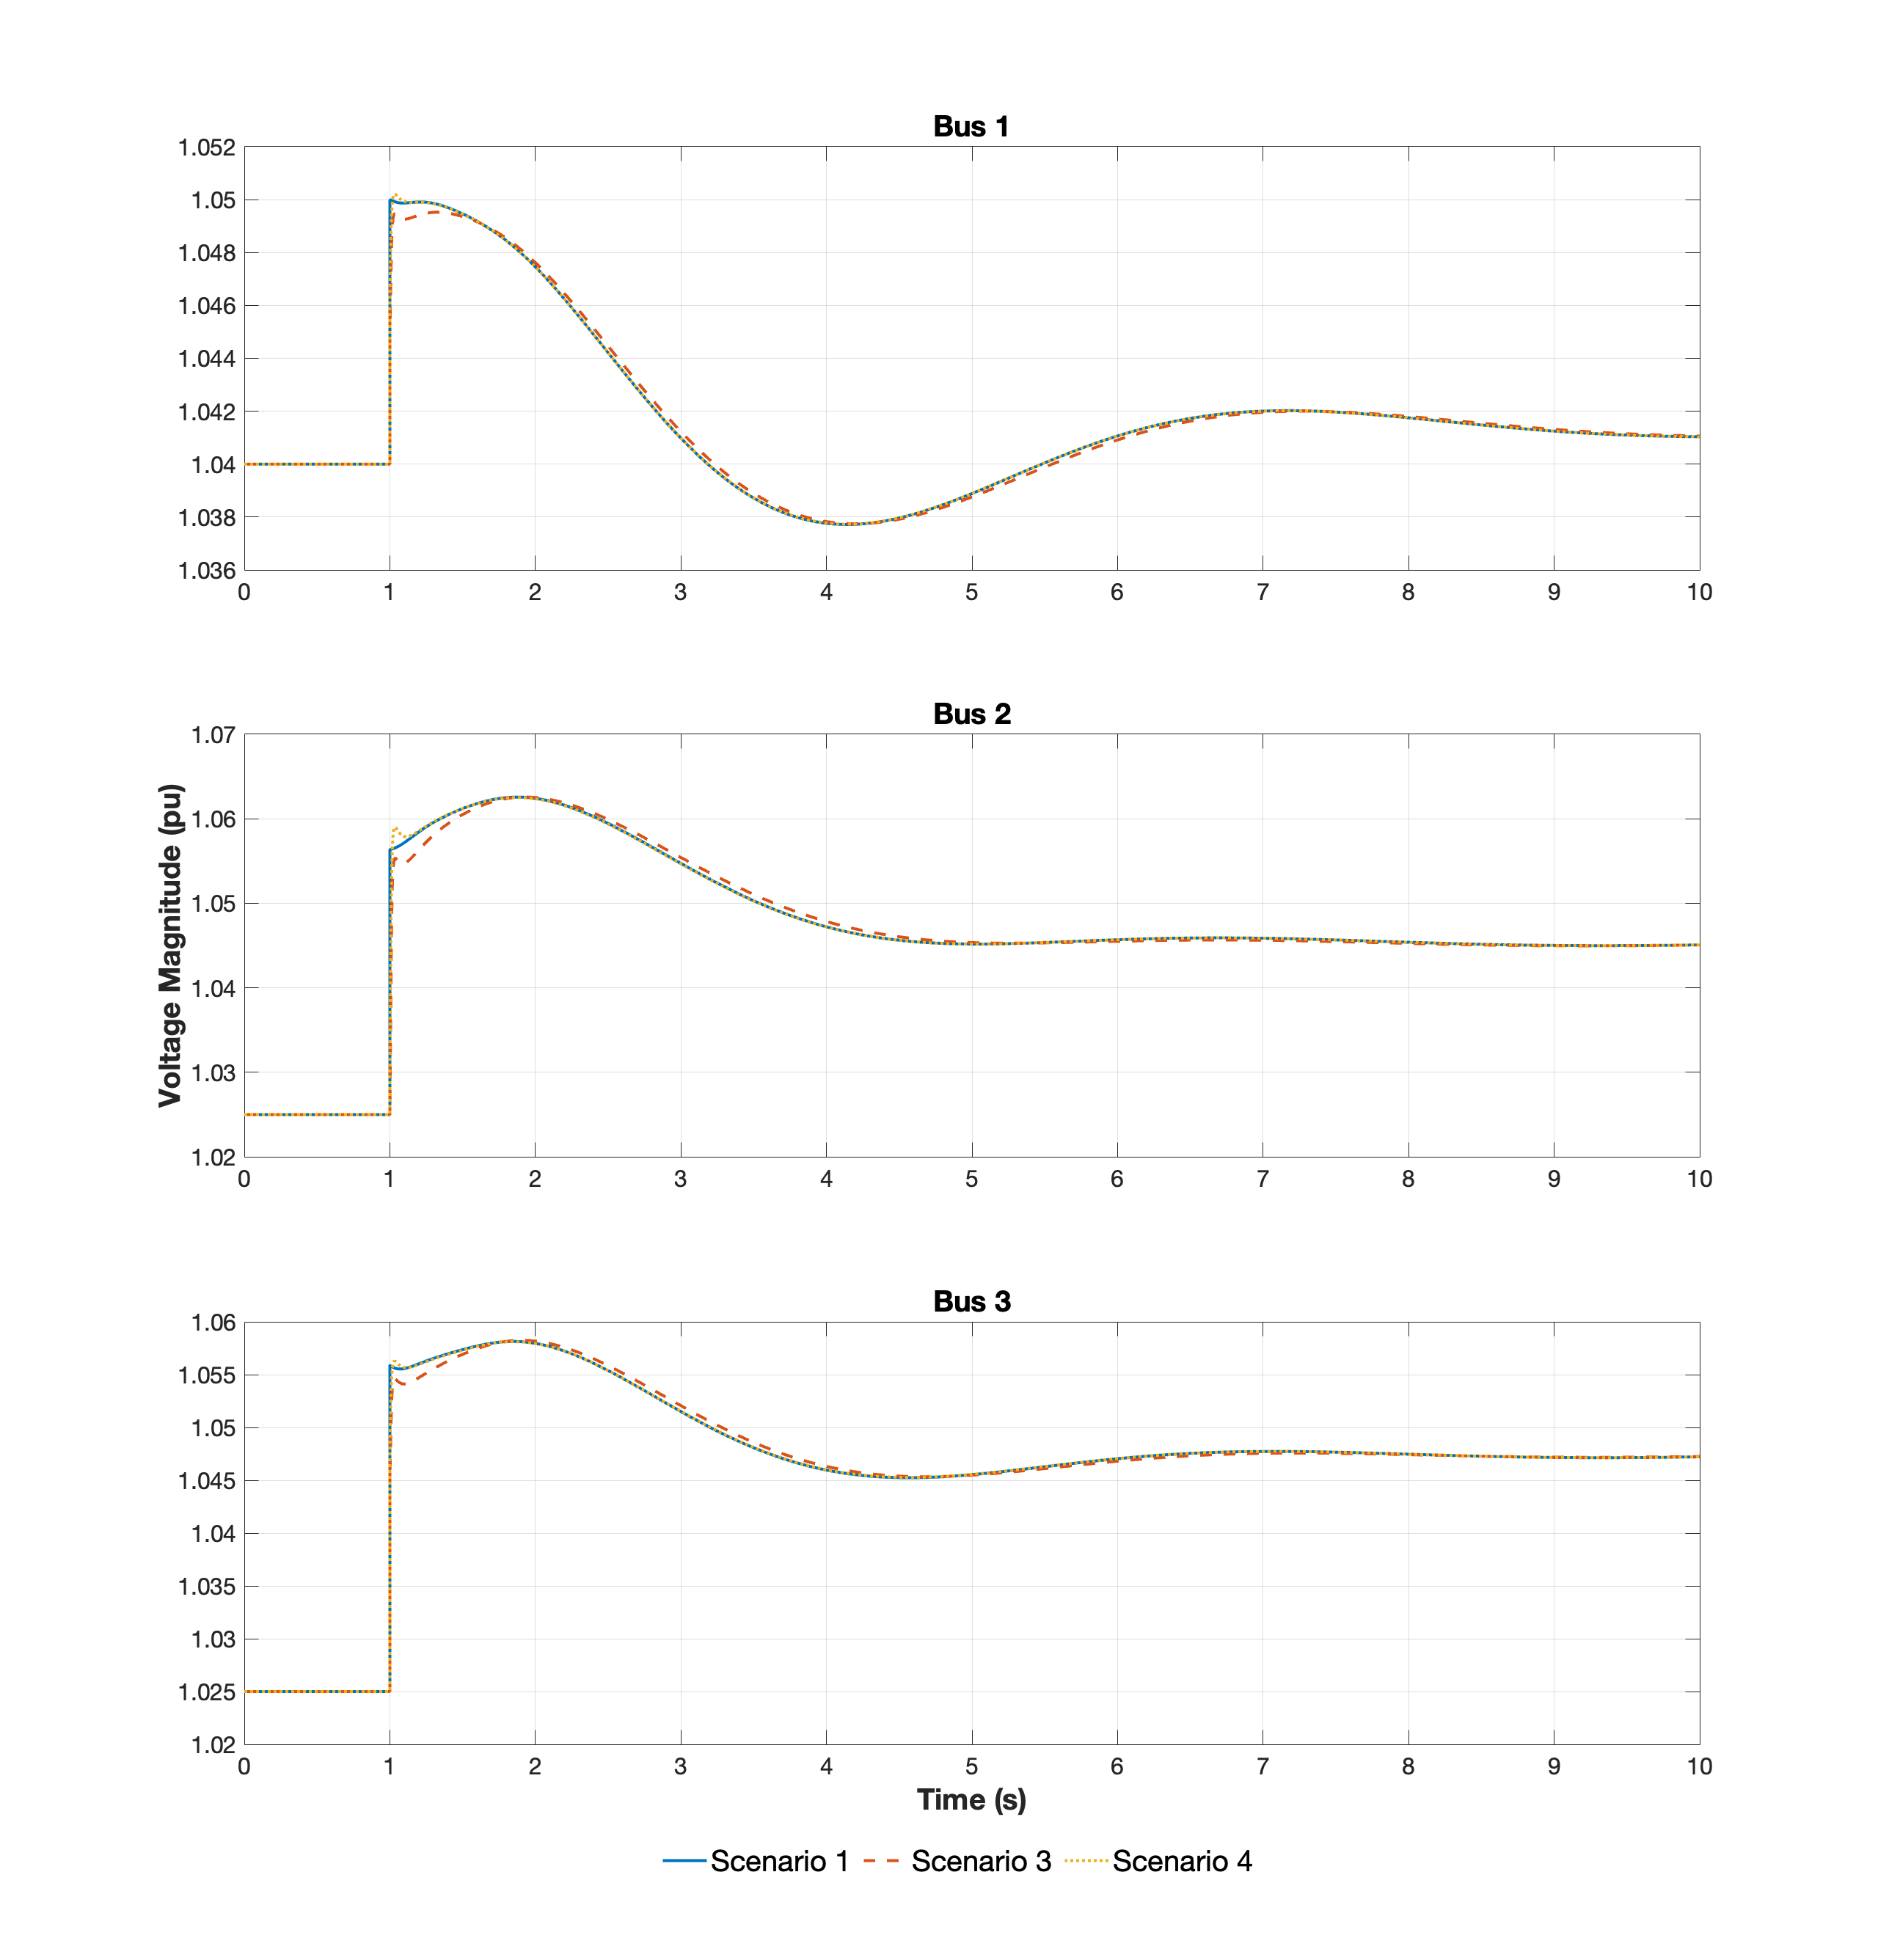
\includegraphics[width = \linewidth]{images/voltage_disconnection.png}
    \caption{Transient reponse to disconnection: voltage magnitude in the generator buses of the four scenarios.}
    \label{fig:voltage_disconnection}
\end{figure}

\newpage
\begin{figure}[ht!]
    \centering
    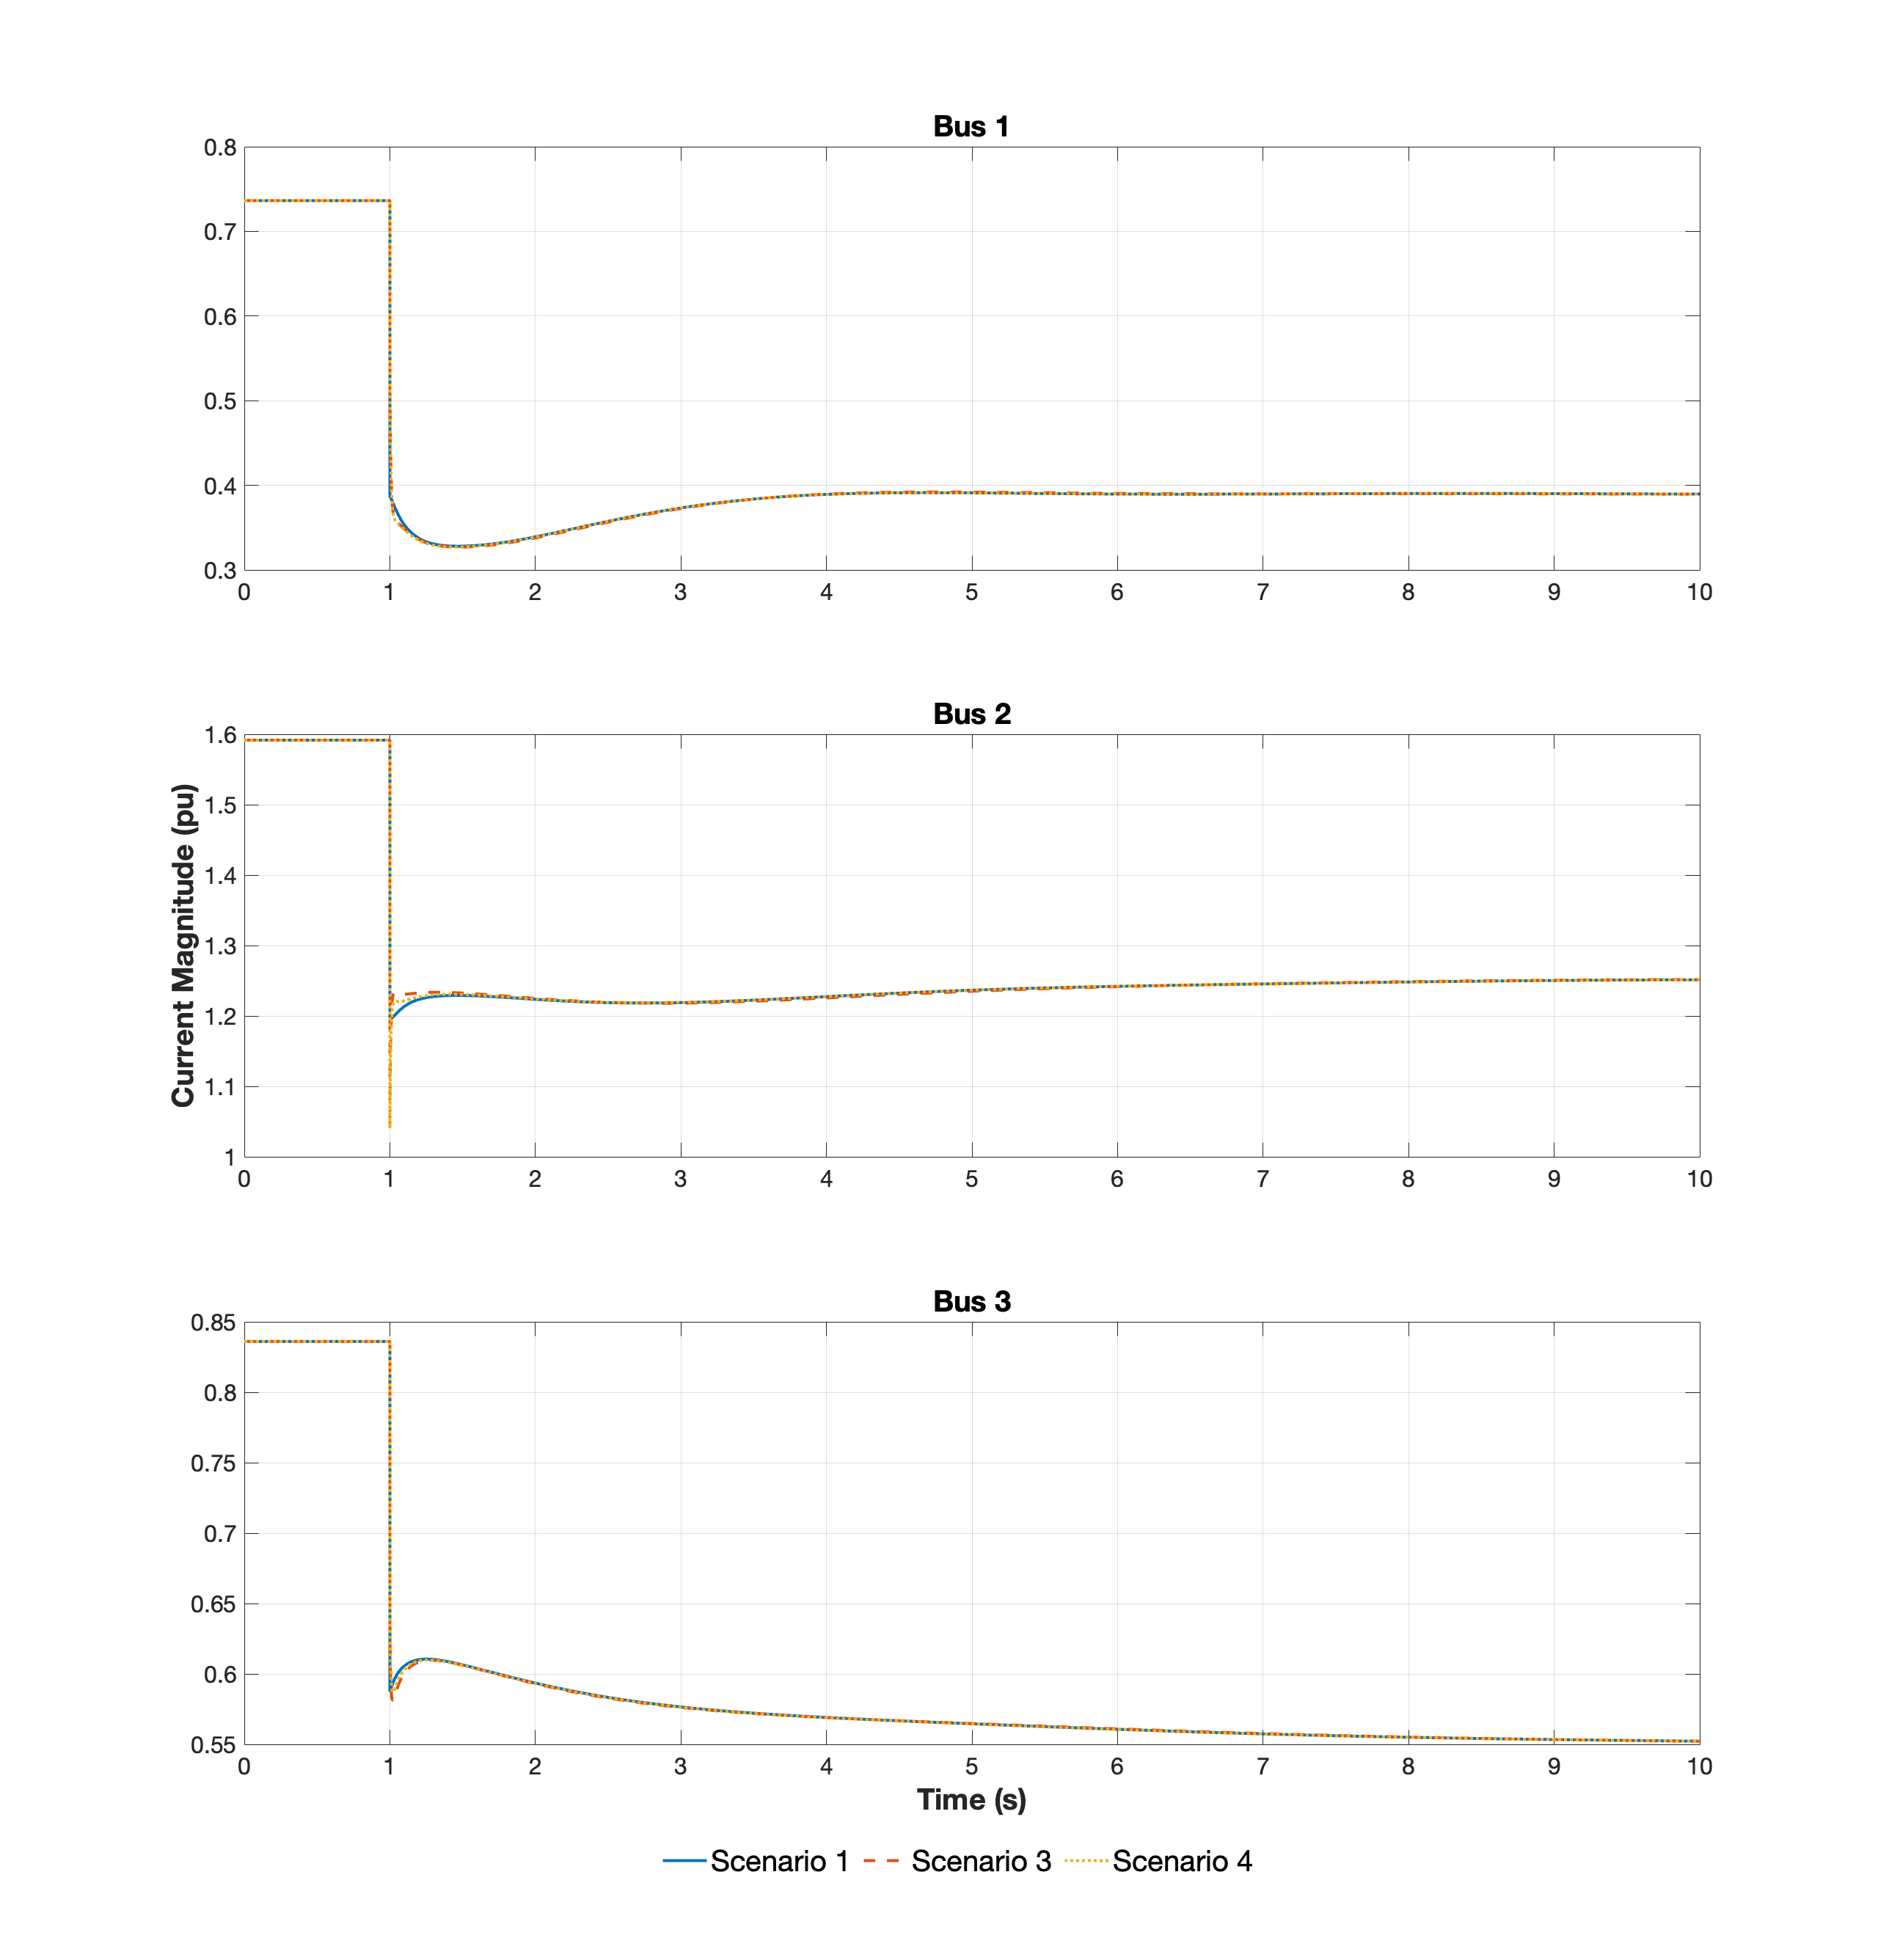
\includegraphics[width = \linewidth]{images/current_disconnection.png}
    \caption{Transient reponse to disconnection: current magnitude in the generator buses of the four scenarios.}
    \label{fig:current_disconnection}
\end{figure}

\newpage
\begin{figure}[ht!]
    \centering
    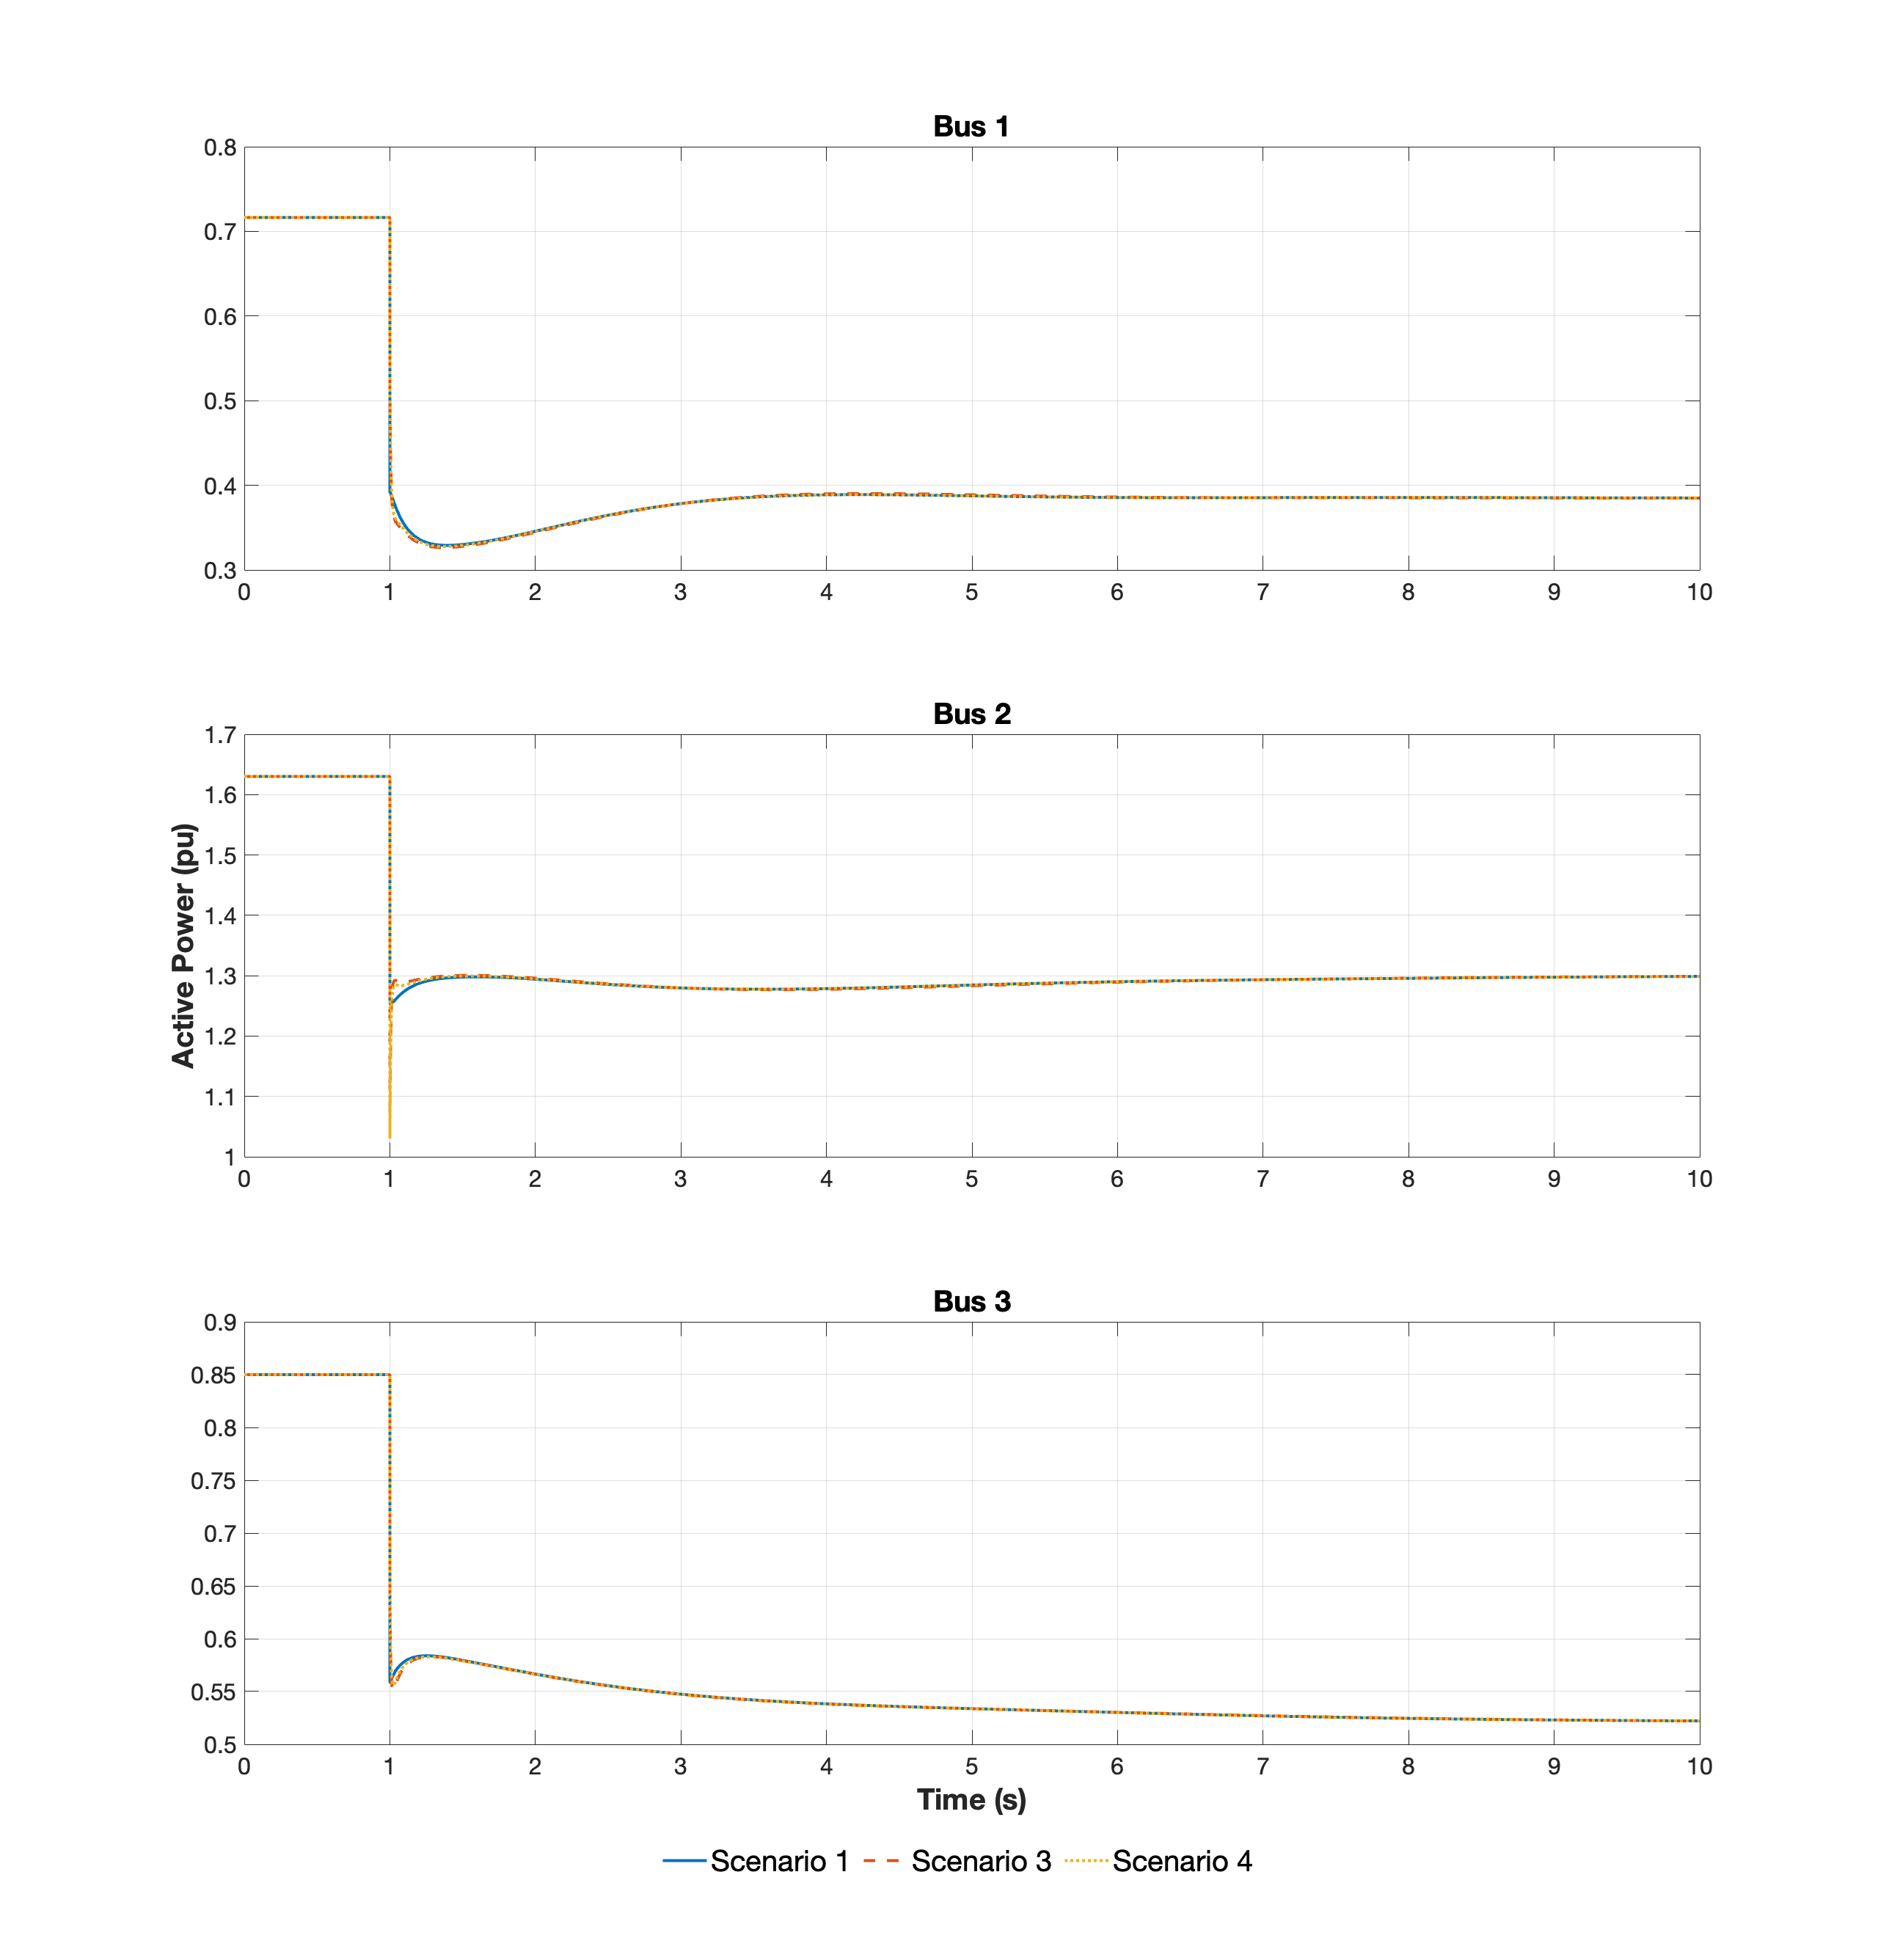
\includegraphics[width = \linewidth]{images/active_disconnection.png}
    \caption{Transient reponse to disconnection: active power in the generator buses of the four scenarios.}
    \label{fig:active_disconnection}
\end{figure}

\newpage
\begin{figure}[ht!]
    \centering
    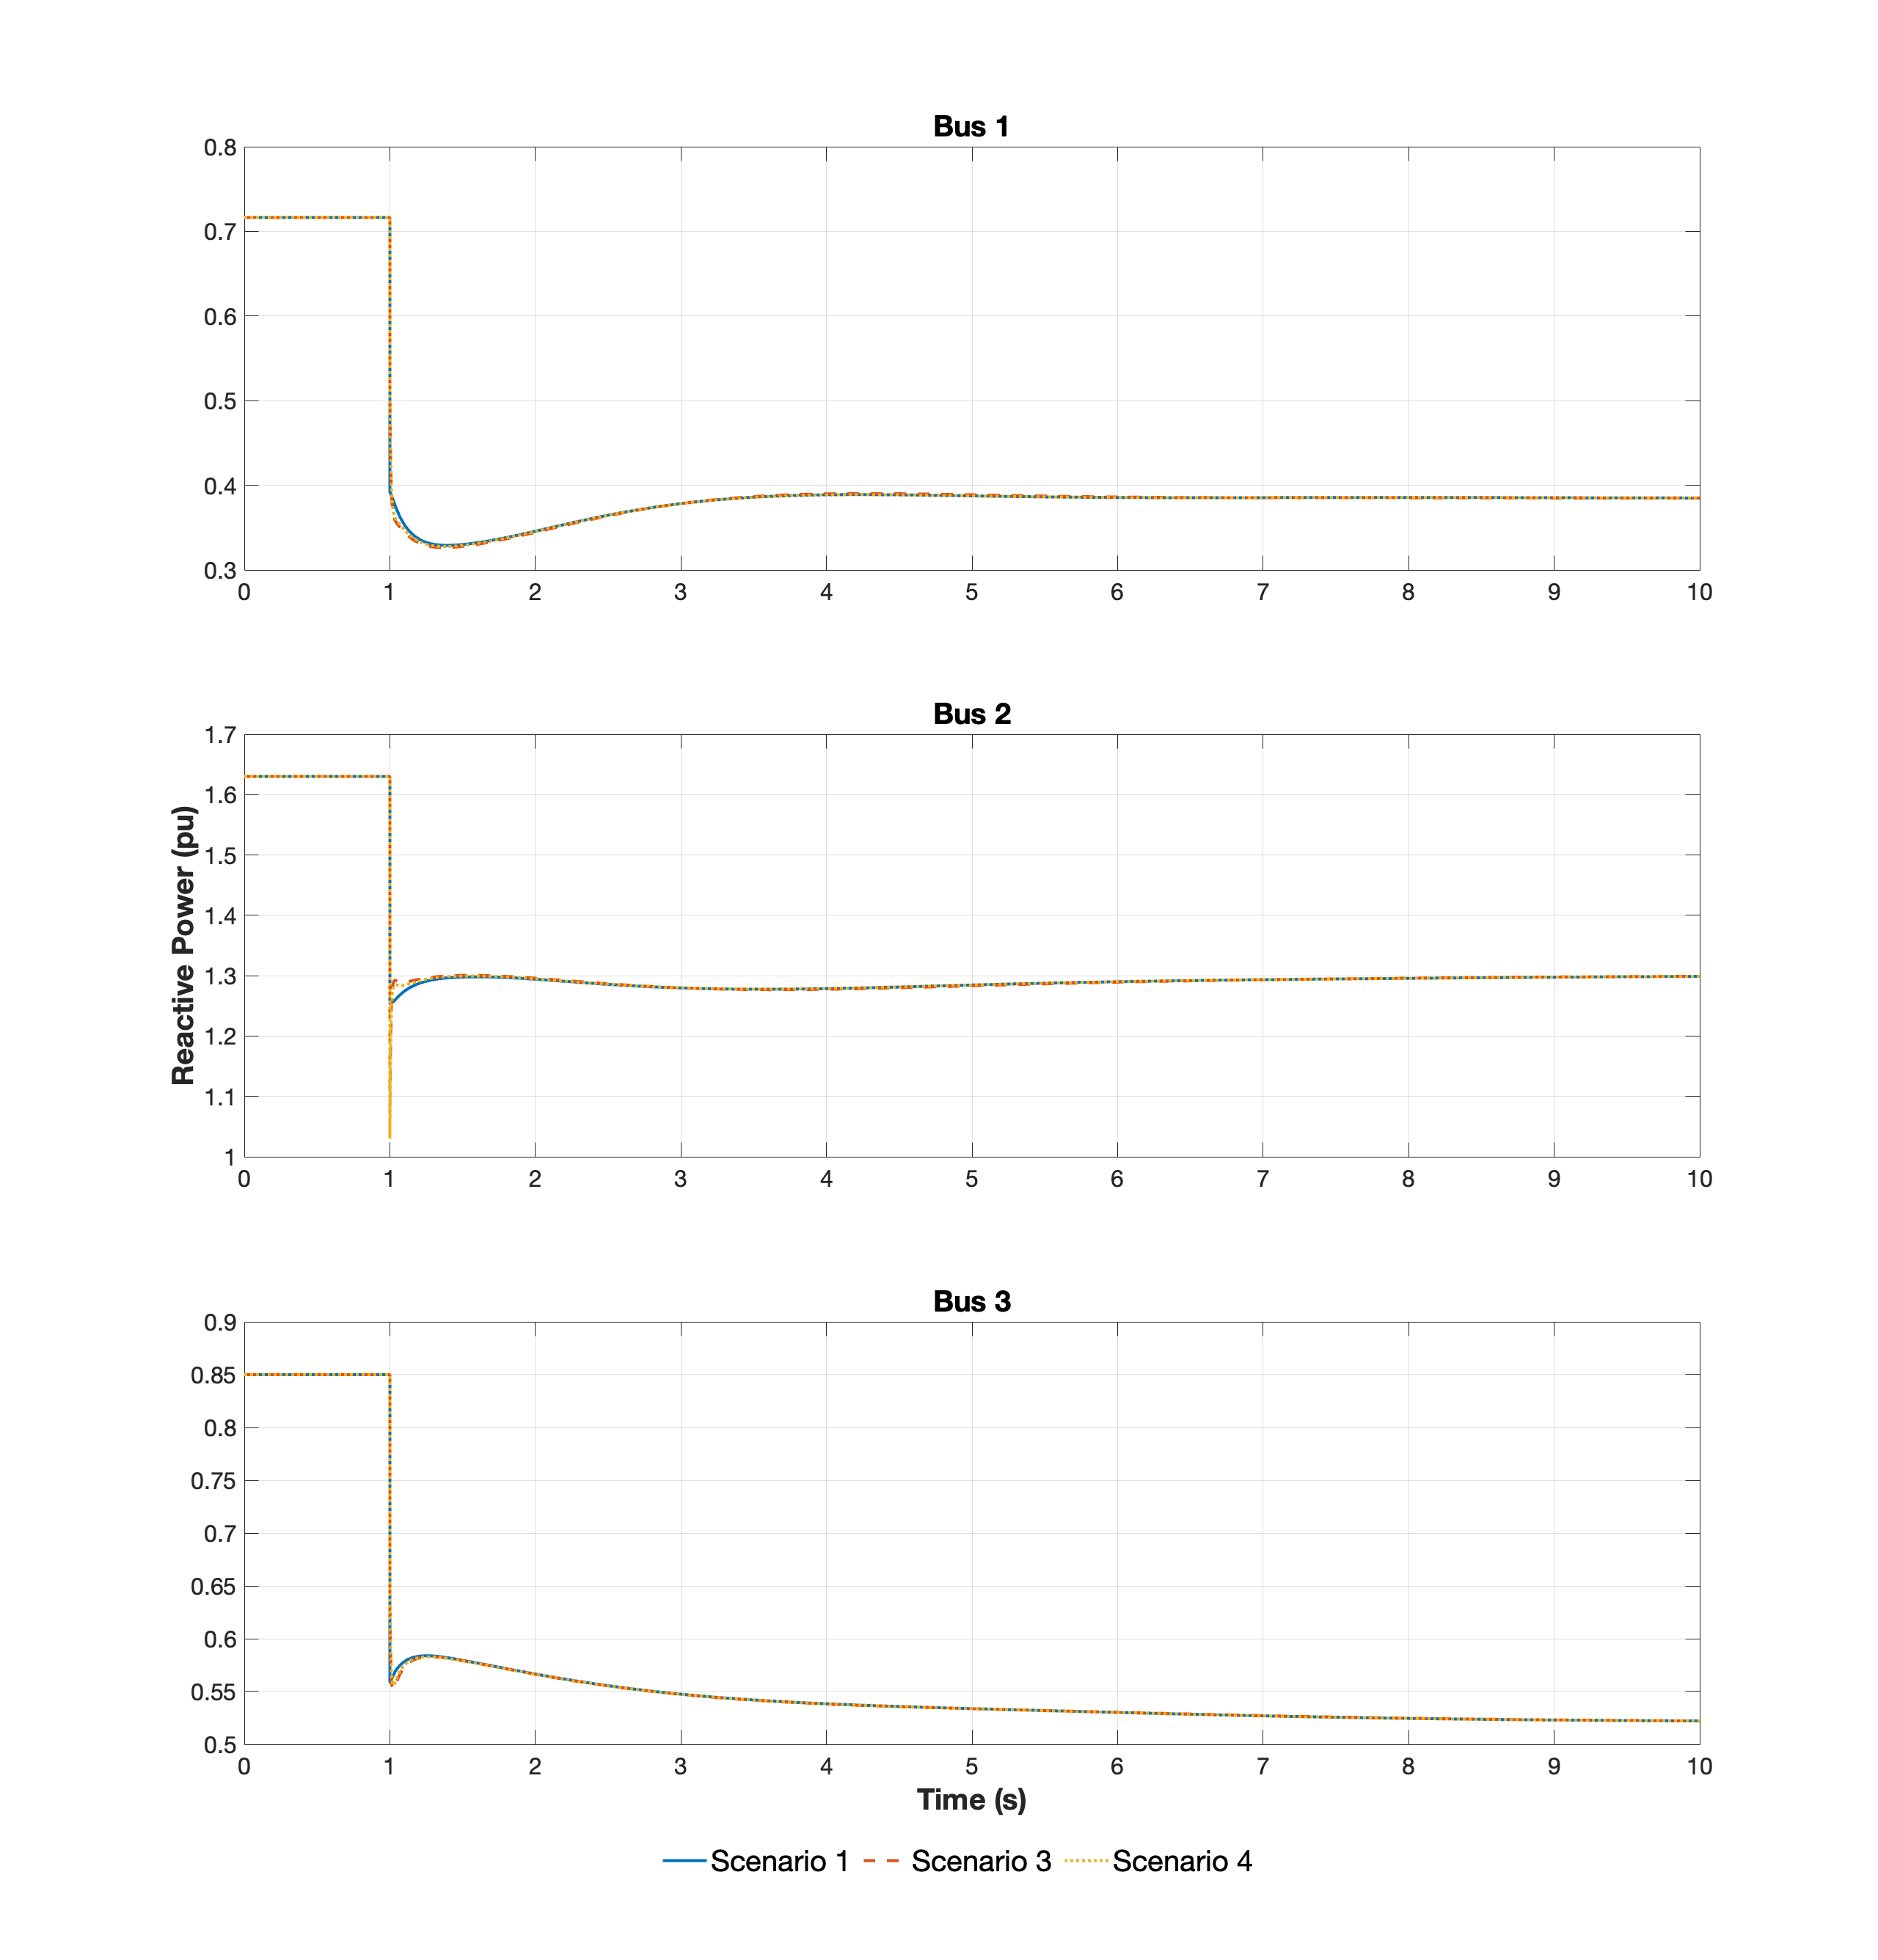
\includegraphics[width = \linewidth]{images/reactive_disconnection.png}
    \caption{Transient reponse to disconnection: reactive power in the generator buses of the four scenarios.}
    \label{fig:reactive_disconnection}
\end{figure}

\section{Effect of Subtransient Reactances}
Since the main difference between the CVSM 1-axis and 2-axis models presented in
this thesis is related to the consideration of the dynamics of the damper
windings, let us investigate how can the parameters related to the damper
windings improve the dynamics of the system. For this purpose, we repeat the
simulation of Section \ref{sec:load_increase} for different values of $X_q'$,
which is the single additional parameter of the 2-axis model in relation to the
1-axis model. For simplification, we analyze only the frequency and voltage
magnitude at the bus 2 (where the CVSM is placed).

\begin{figure}[ht!]
    \centering
    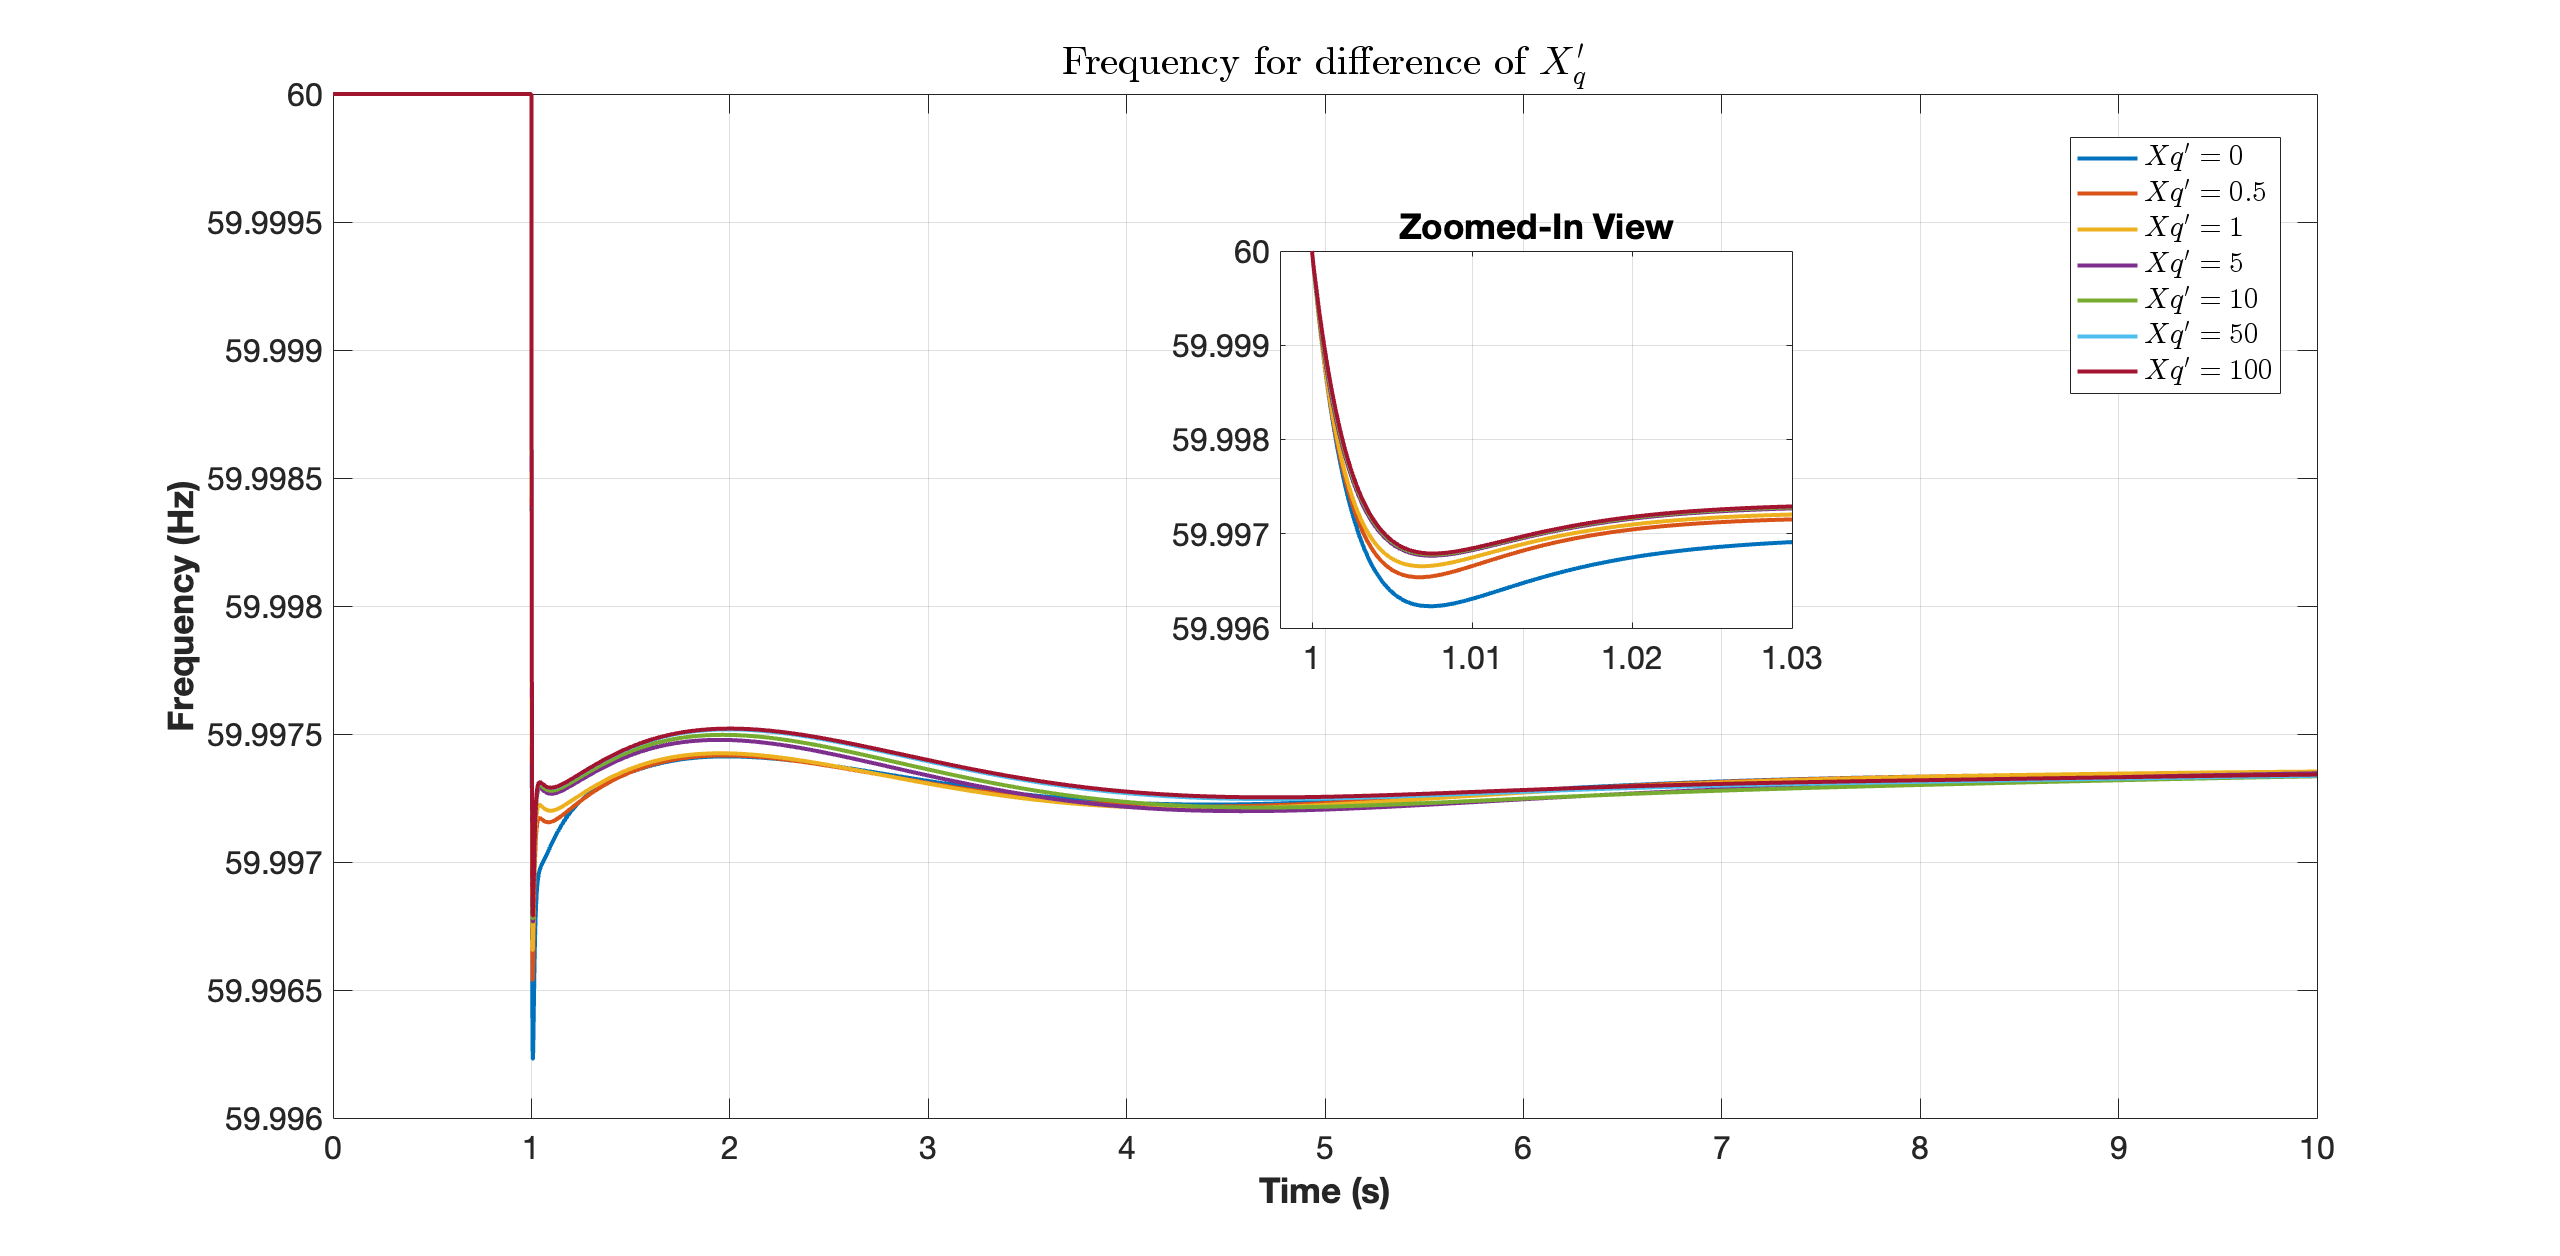
\includegraphics[width = \linewidth]{images/omega_varying.png}
    \caption{Frequency at bus 2 for different values of $X_q'$}
    \label{fig:omega_varying}
\end{figure}

\begin{figure}[ht!]
    \centering
    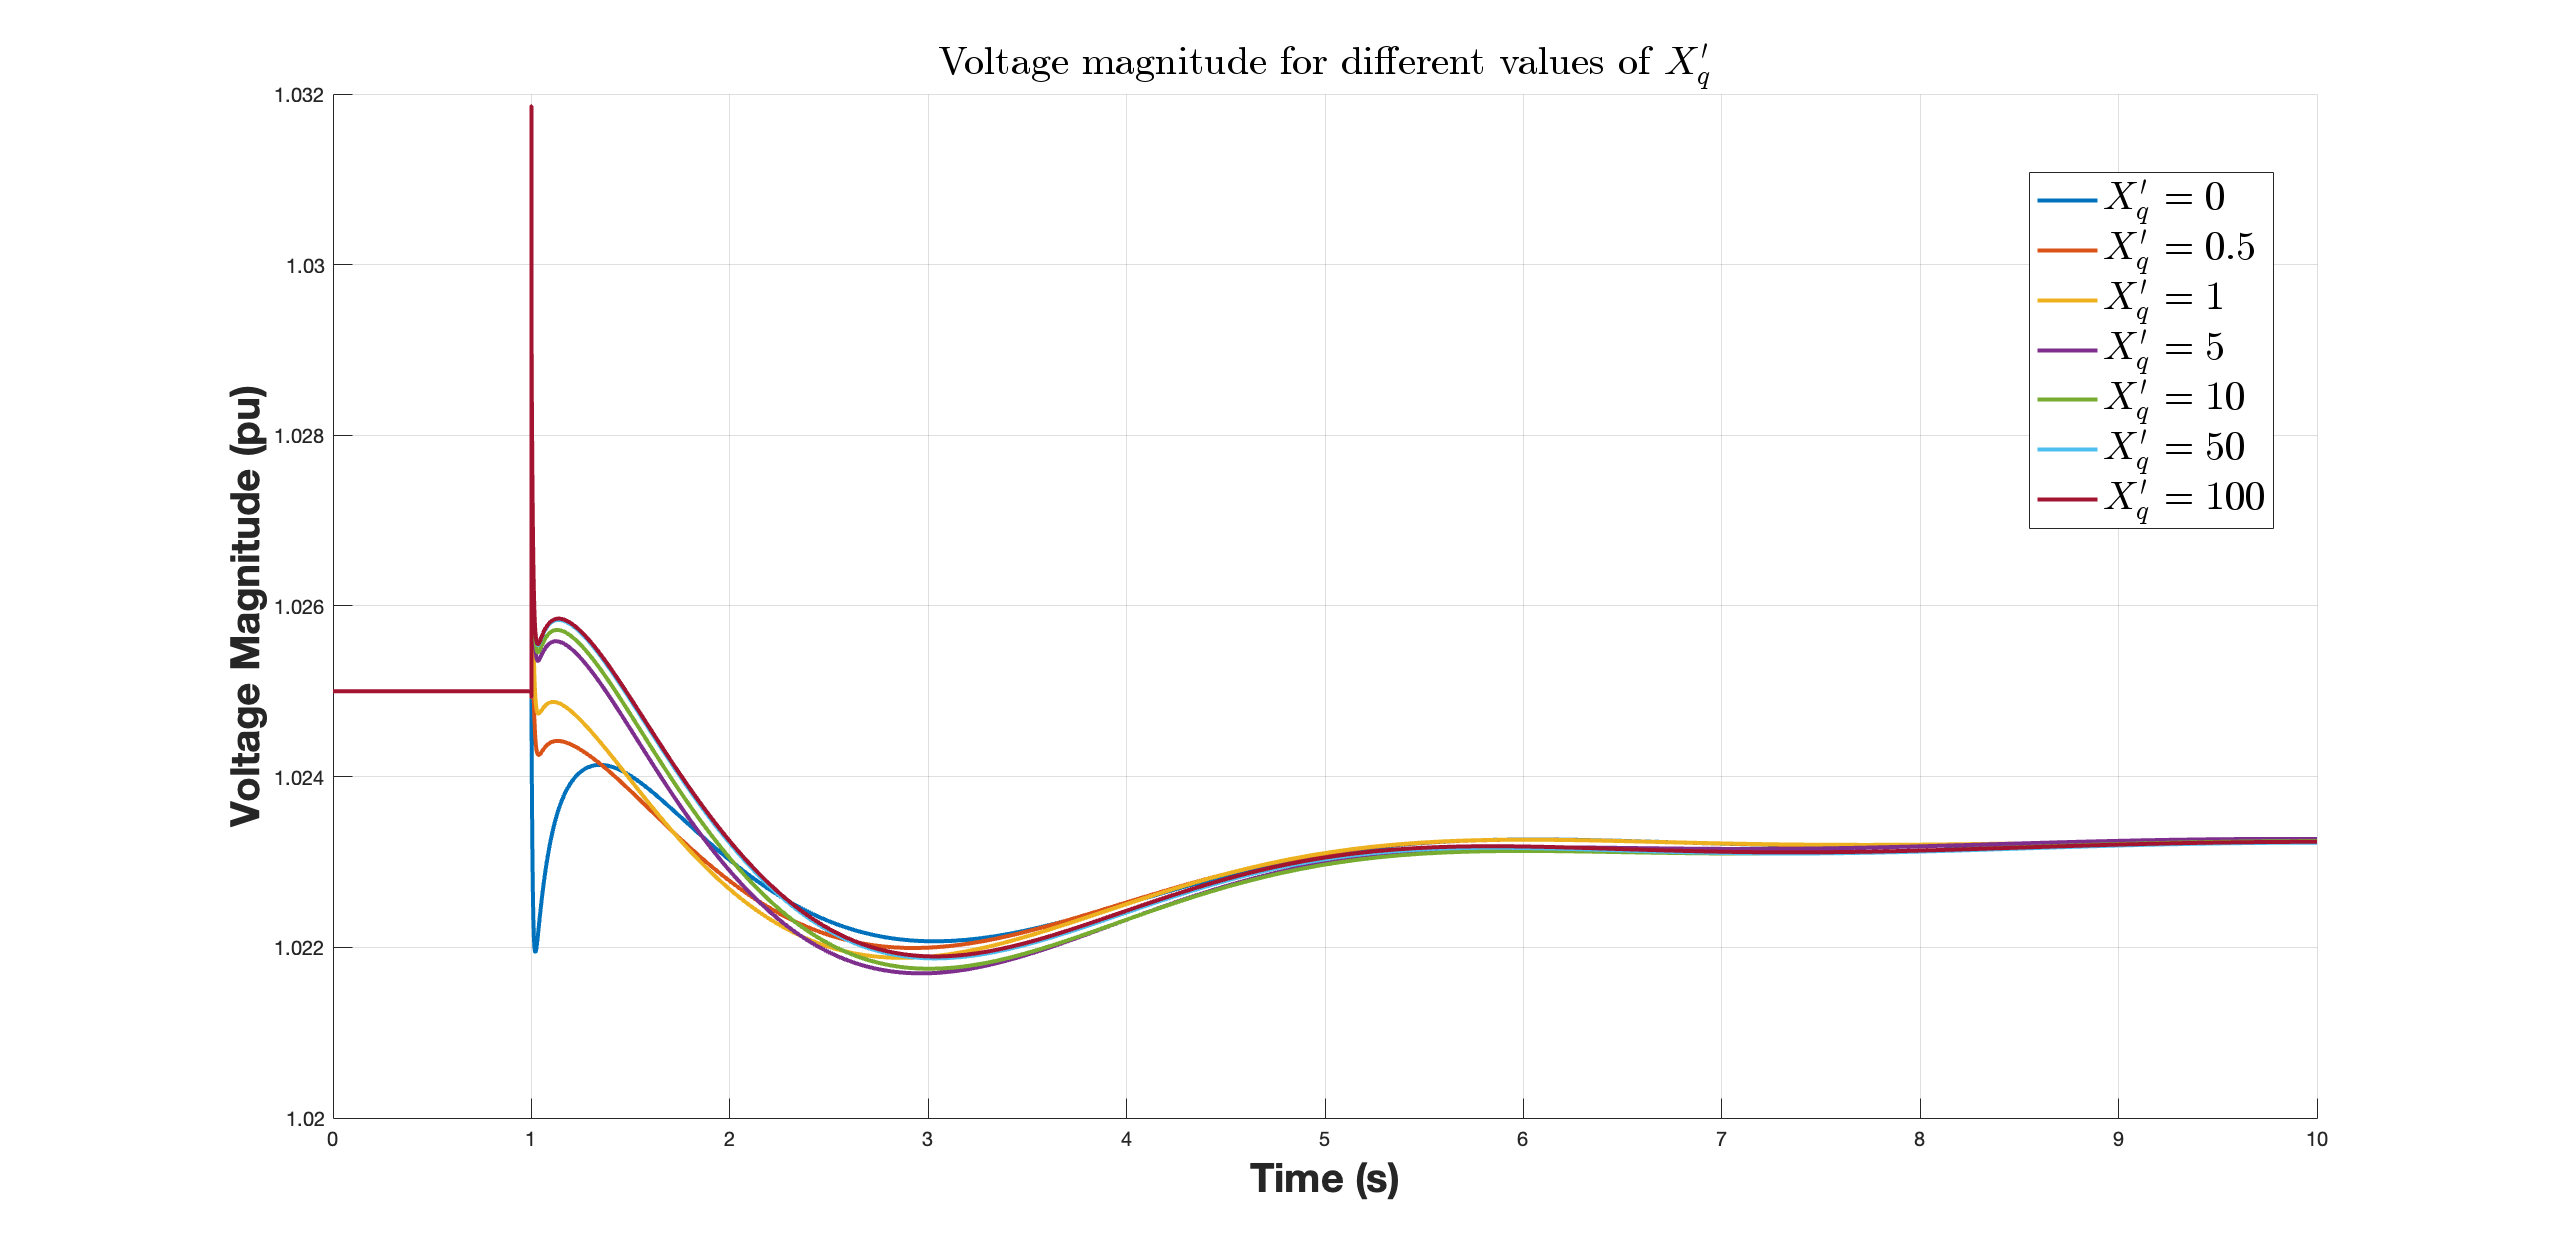
\includegraphics[width = \linewidth]{images/voltage_varying.png}
    \caption{Voltage magnitude at bus 2 for different values of $X_q'$}
    \label{fig:voltage_varying}
\end{figure}

From Figures \ref{fig:omega_varying} and \ref{fig:voltage_varying}, we conclude
that variations in $X_q'$ have an impact in the transient response of the
system, meaning that the 2-axis model has one additional degree of freedom for
improving the system dynamics when comparing with the 1-axis model. However, the
effects of $X_q'$ is not too significant, given that large variations results in
small changes in the transient response. Therefore, we conclude that the
differences between the CVSM with 1-axis model is enough for providing a
sufficiently good dynamic response.

However, as discussed in Section \ref{sec:load_increase}, the CVSM with
classical model has a much worse performance, and could not even handle the
disturbances discussed in Section \ref{sec:disconnection}. Since the difference
between these two models is related to the consideration of an exciter winding,
in Figures \ref{fig:omega_varying2} and \ref{fig:voltage_varying2} we show that
variations in $X_d'$, which is the single additional parameter of the 1-axis
model in relation to the classical model, can drastically impact the system
dynamics.

\begin{figure}[ht!]
    \centering
    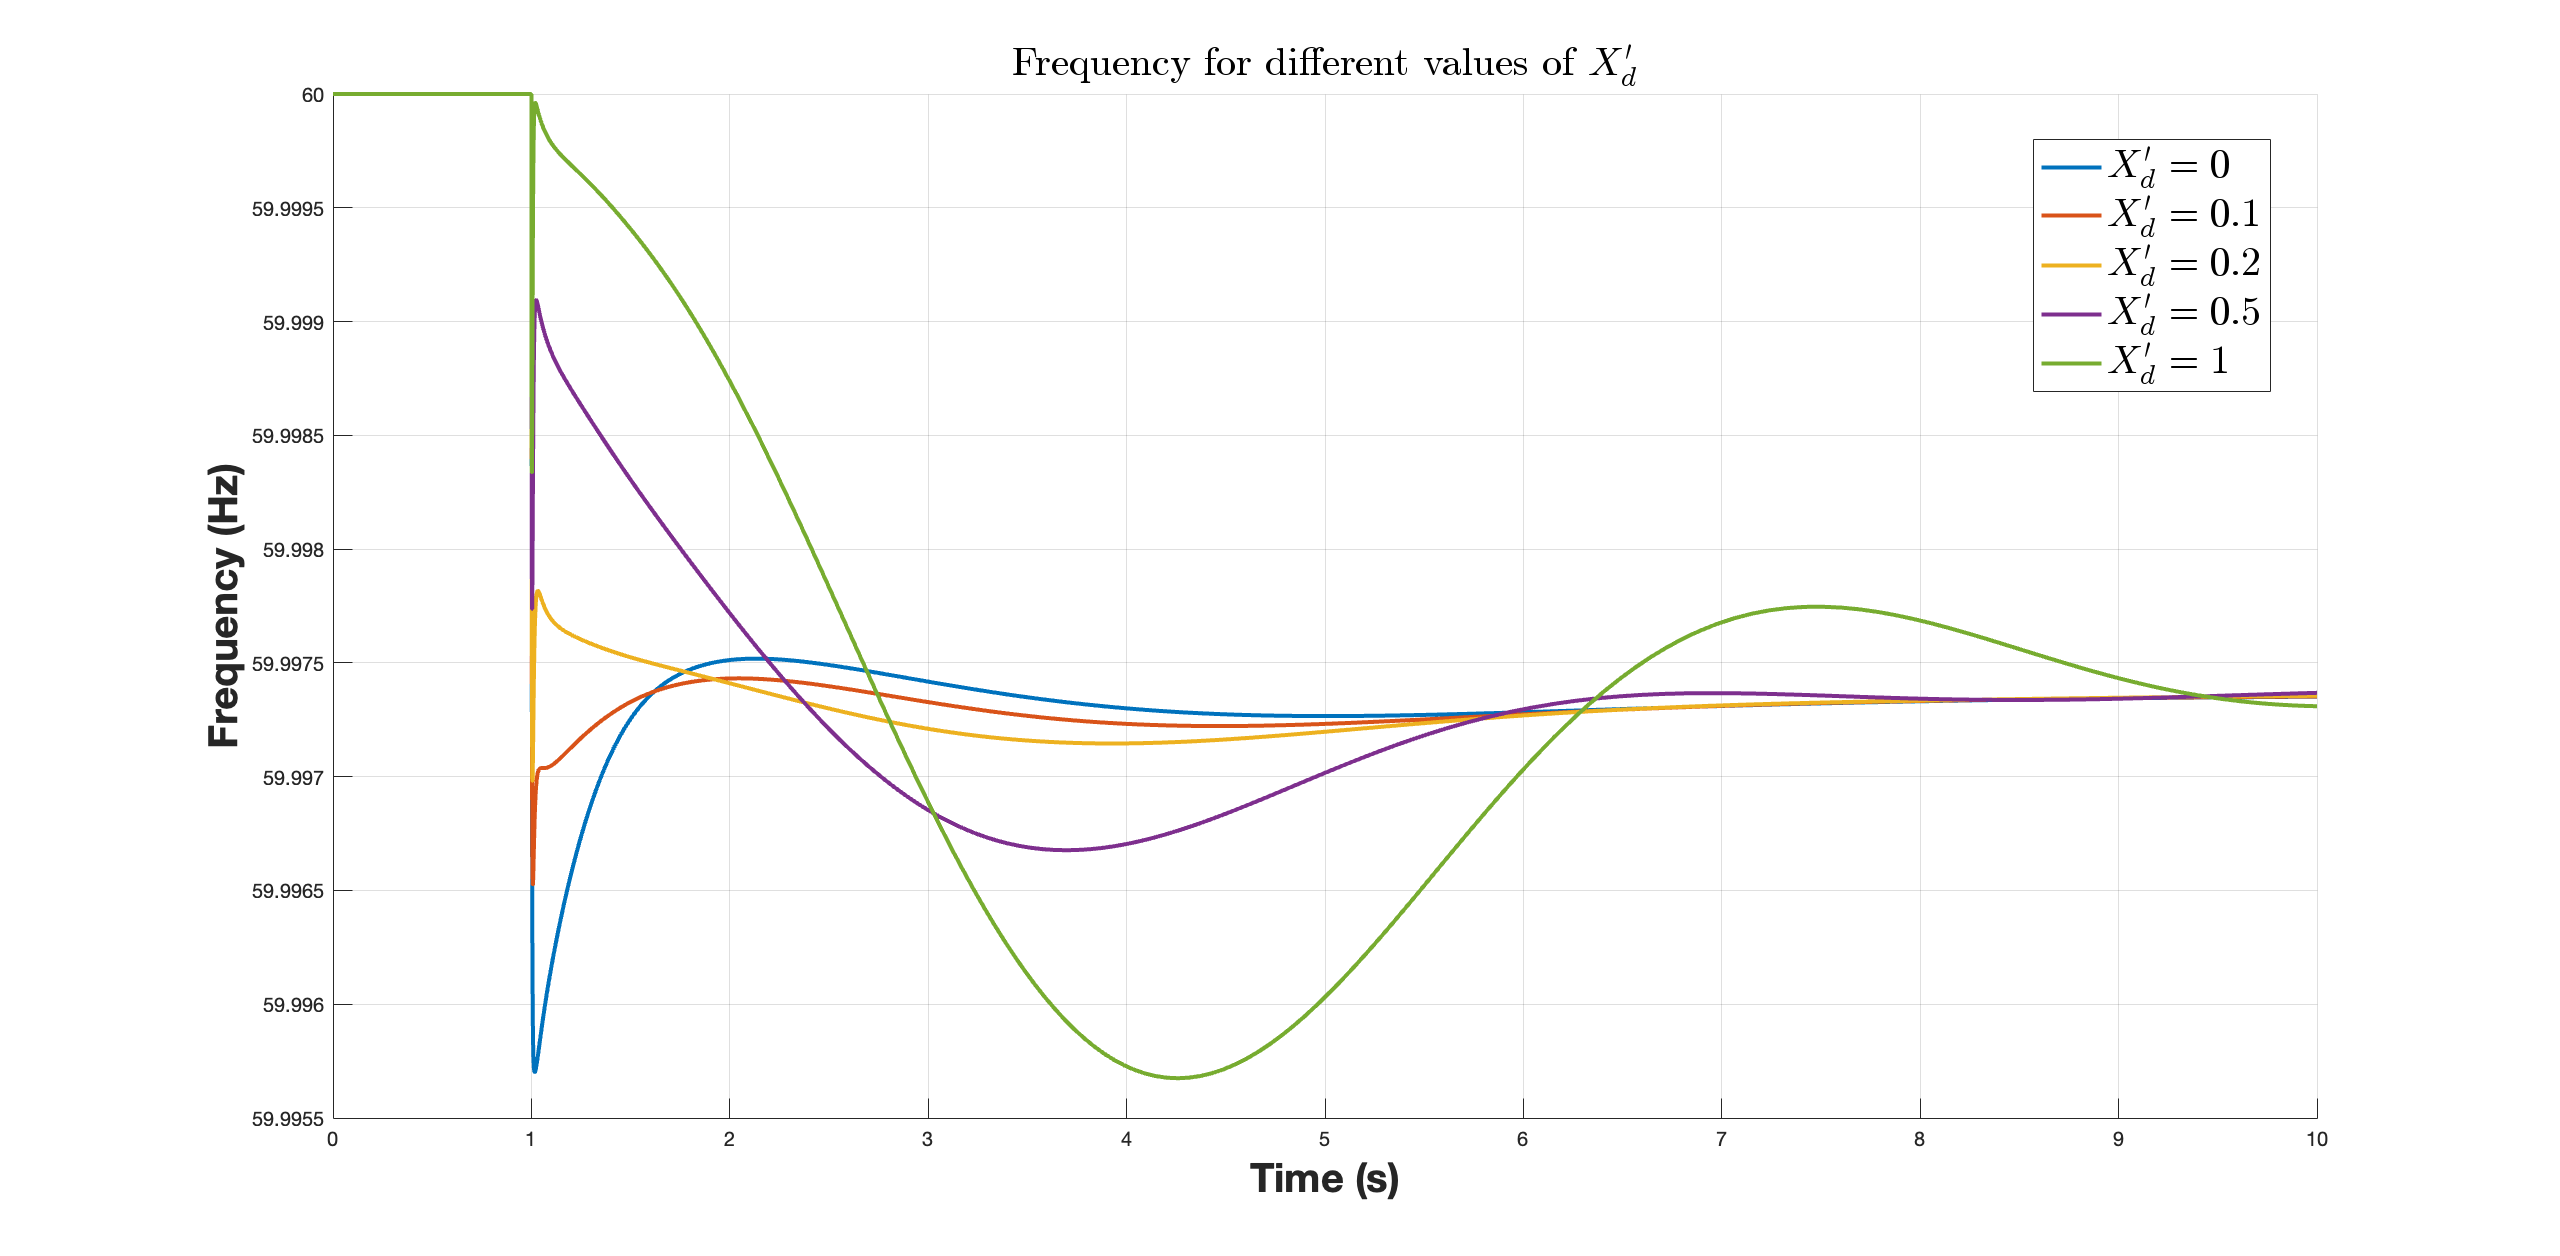
\includegraphics[width = \linewidth]{images/omega_varying2.png}
    \caption{Frequency at bus 2 for different values of $X_d'$}
    \label{fig:omega_varying2}
\end{figure}

\begin{figure}[ht!]
    \centering
    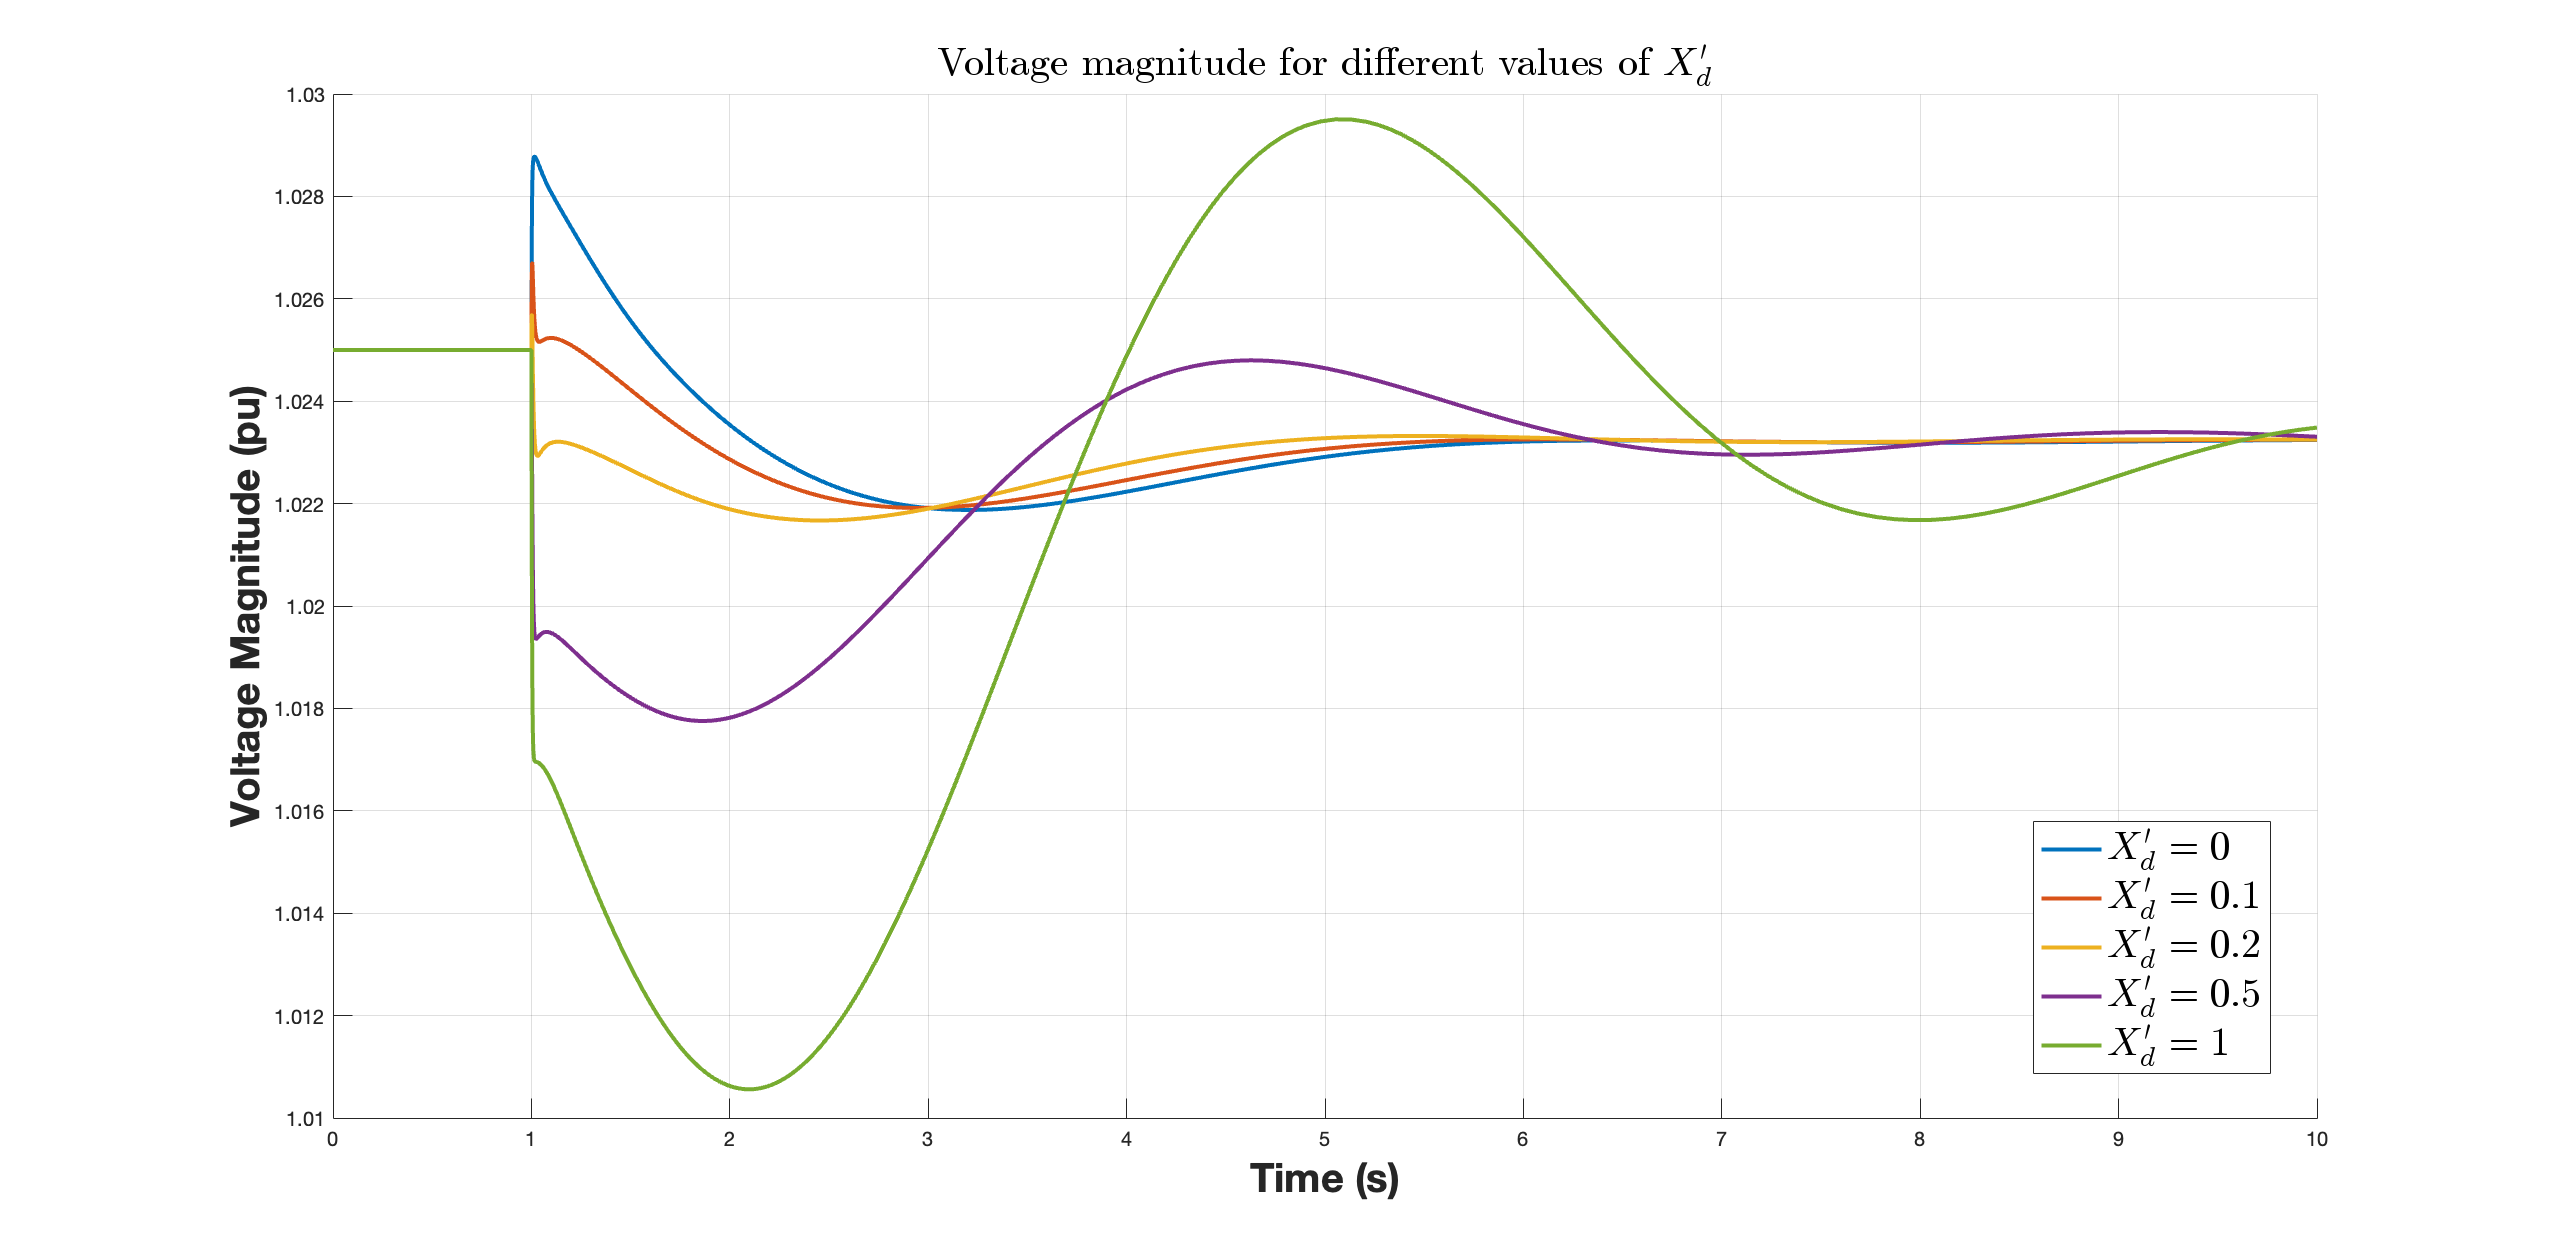
\includegraphics[width = \linewidth]{images/voltage_varying2.png}
    \caption{Voltage magnitude at bus 2 for different values of $X_d'$}
    \label{fig:voltage_varying2}
\end{figure}